\documentclass[10pt,letterpaper]{article}
\usepackage[T1]{fontenc}
\usepackage[utf8]{inputenc}
\usepackage{lmodern}
\usepackage[margin=0.65in,headheight=14pt,headsep=12pt,footskip=24pt]{geometry}
\usepackage{microtype}
\usepackage{graphicx}
\usepackage{float}
\usepackage{booktabs,tabularx,array}
\usepackage{xcolor}
\usepackage{multicol}
\usepackage{enumitem}
\usepackage{caption}
\usepackage{fancyhdr}
\usepackage{titlesec}
\usepackage{xurl}
\usepackage{hyperref}
\definecolor{surveyblue}{HTML}{0056B3}
\definecolor{surveyred}{HTML}{C52214}
\definecolor{surveyblack}{HTML}{18171C}
\hypersetup{colorlinks=true,linkcolor=surveyblue,urlcolor=surveyblue,
 pdftitle={Human Body Communication: A Living Survey of Integrated Circuits and Channel Models},
 pdfauthor={Shreyas Sen},pdfsubject={v3.11, 13 November 2026; publication catalogue and IC energy-efficiency plots; 13 November 2026 snapshot},
 bookmarksnumbered=true}
\urlstyle{same}
\titleformat{\section}{\large\bfseries\color{surveyblue}}{\thesection}{.65em}{}
\titlespacing*{\section}{0pt}{11pt}{5pt}
\captionsetup{font=small,labelfont=bf,skip=5pt}
\pagestyle{fancy}
\fancyhf{}
\fancyhead[L]{\small\color{surveyblack}Human Body Communication: A Living Survey}
\fancyhead[R]{\small\color{surveyblack}v3.11 / 13 November 2026}
\fancyfoot[C]{\small\thepage}
\renewcommand{\headrulewidth}{0.3pt}
\setlength{\parindent}{0pt}
\setlength{\parskip}{5pt}
\setlength{\columnsep}{19pt}
\setlength{\emergencystretch}{2em}
\newcolumntype{Y}{>{\raggedright\arraybackslash}X}
\newcommand{\snapshot}{13 November 2026}
\newcommand{\website}{\href{https://engineering.purdue.edu/~shreyas/SparcLab/HBC_Survey.html}{SparcLab HBC survey website}}
\newcommand{\cataloguefont}{\fontsize{8.3}{9.5}\selectfont\setlength{\parskip}{2.2pt}\raggedright}
\newcommand{\entry}[4]{\par\noindent\begin{minipage}{\linewidth}\raggedright\hypertarget{#2}{}\textbf{\color{surveyred}[#1]}\enspace #3. #4\end{minipage}\par}

\begin{document}
\thispagestyle{plain}
\begin{center}
{\LARGE\bfseries\color{surveyblack}Human Body Communication:\\[5pt]
A Living Survey of Integrated Circuits\\[5pt]
and Channel Models\par}
\vspace{10pt}
% Confirm the author list before submission; acknowledgements do not determine authorship.
{\large Shreyas Sen}\par
{\small Elmore Family School of Electrical and Computer Engineering\\
Purdue University, West Lafayette, Indiana, USA}\par
\vspace{3pt}
{\small v3.11\quad\textbar\quad 13 November 2026\quad\textbar\quad Literature snapshot: \snapshot}
\end{center}
\vspace{2pt}
\begin{abstract}
This manuscript provides a fixed, searchable edition of the SparcLab human body communication (HBC) literature catalogue. Its purpose is to collect the publications in one place and make progress in integrated-circuit (IC) energy efficiency visible through publication-year plots. The \snapshot\ snapshot contains 337 records: 103 IC publications, 147 channel/model publications, and 87 other references. All records are listed in a compact bibliography with stable identifiers and source links where available. IC plots begin in 2006, the earliest year represented in the IC collection, and display transmitter, receiver, and combined transmitter--receiver energy separately. Machine-readable bibliographic and measurement files accompany the manuscript. The resource supports publication discovery and inspection of archived IC performance data.
\end{abstract}

\section{The catalogue at a glance}
The catalogue brings together the records maintained by the \website. Readers can search the PDF by title, first author, venue, year, or record identifier, and follow a linked title or DOI to its source. The accompanying data retain full stored author strings, additional source links, and measurement notes. Table~\ref{tab:totals} reports the total collection sizes.

\begin{table}[h]
\centering\small
\caption{Total records in the \snapshot\ catalogue.}
\label{tab:totals}
\begin{tabularx}{.94\linewidth}{@{}YrY@{}}
\toprule
Collection & Records & Location in this manuscript\\
\midrule
Integrated circuits & 103 & Section~\ref{cat:ic}\\
Channels and models & 147 & Section~\ref{cat:channel}\\
Other literature & 87 & Section~\ref{cat:other}\\
\midrule
\textbf{Total} & \textbf{337} & Complete catalogue\\
\bottomrule
\end{tabularx}
\end{table}

\begin{figure}[h]
\centering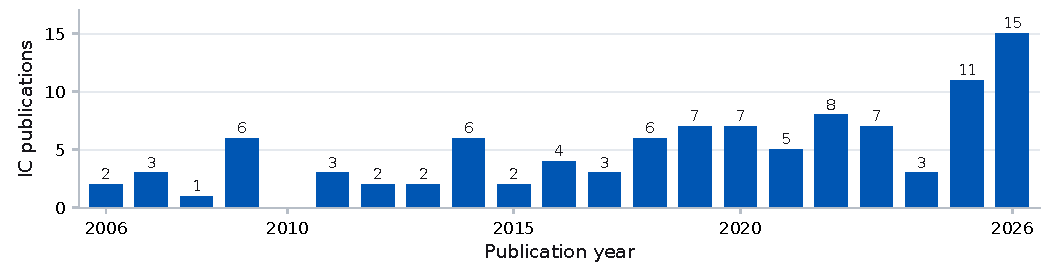
\includegraphics[width=.96\linewidth]{figures/ic_publications.pdf}
\caption{IC publication counts by stored publication year, starting with the earliest included IC papers in 2006. Counts total 103 publications; conference and journal reports are counted as separate records when both are retained. The 2026 count covers the snapshot through \snapshot.}
\label{fig:counts}
\end{figure}

The collection includes HBC and related body-area/implant literature. Its three categories support finding papers; only records classified as eligible fabricated custom solid-state ICs enter the comparison plots. These are counts of publications, not counts of unique chips. The catalogue is a curated collection and does not claim exhaustive coverage of the field.

\clearpage
\section{IC energy efficiency over time}
Figure~\ref{fig:energy} provides a visual record of the energy values in the IC collection. Each point is a stored operating point; one publication can contribute more than one point. Lower energy per bit indicates greater energy efficiency within the stated measurement scope.
\begin{figure}[H]
\centering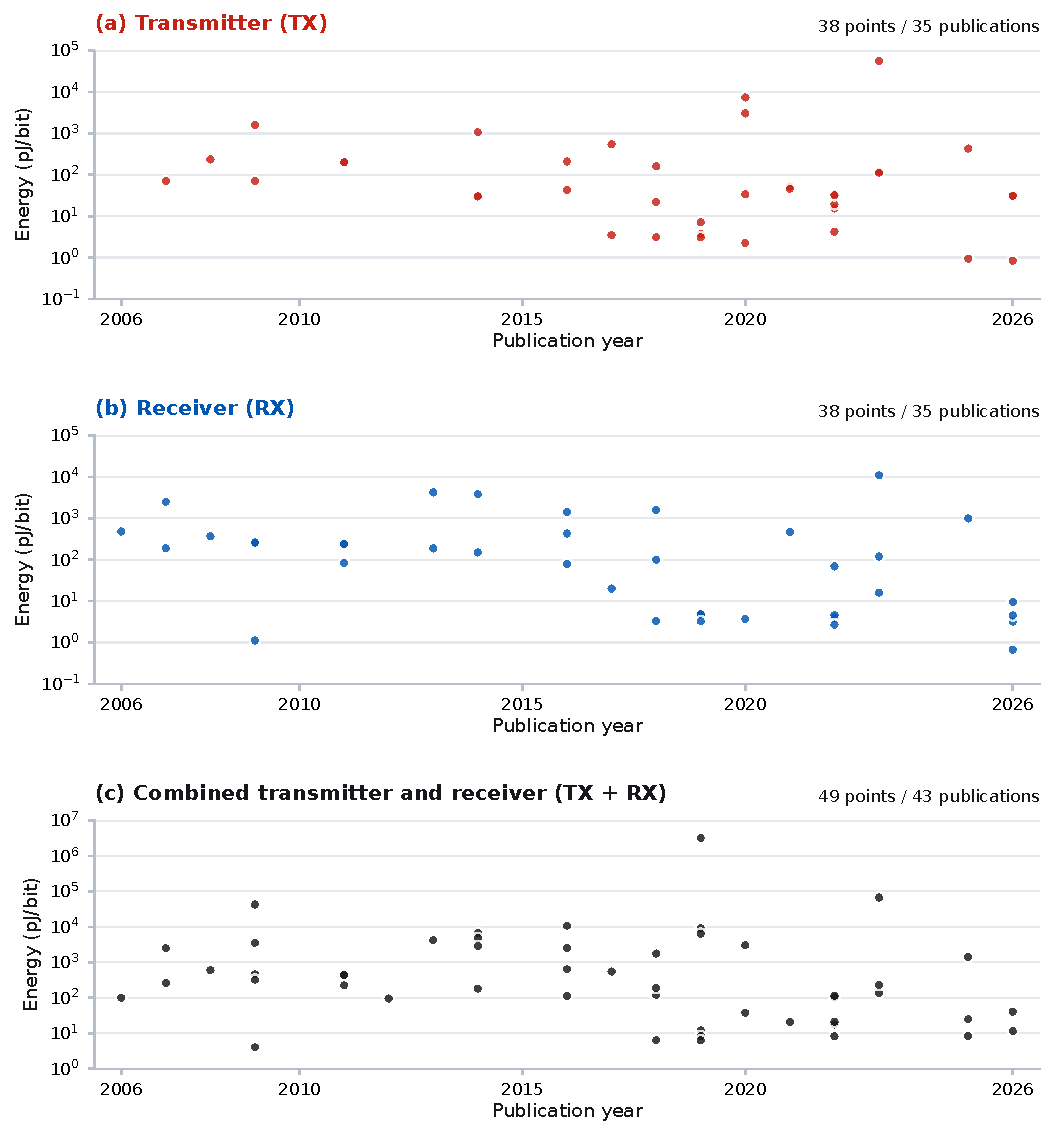
\includegraphics[width=.92\linewidth]{figures/ic_energy.pdf}
\caption{Archived IC energy per bit versus publication year: (a) TX, (b) RX, and (c) TX+RX. The plots use positive numeric entries from the same eligible IC records as the website. Vertical axes are logarithmic and have panel-specific ranges. Combined values are those reported or explicitly calculated in the archive. Missing values are omitted; separate panels can therefore contain different publications. Overlapping points can conceal one another. Source identifiers and values for every plotted point are supplied in \texttt{anc/energy\_points.csv}.}
\label{fig:energy}
\end{figure}

\clearpage
\small
\section{Using and citing this edition}
\textbf{Reading the plots.} The plots retain stored energy scopes, operating conditions, and publication years. The IC archive includes adjacent body-area and implant modalities as well as electrical HBC. Data rates, component exclusions, and link configurations differ between papers; consult the original publications and record notes before making a quantitative comparison. No trend fit or performance ranking is imposed. Four inherited combined-energy entries (158, 184, 186, 303) are withheld because the stored total is below a listed component value. Original values are retained in the data pending source reconciliation.

\textbf{Finding a paper and its data.} Sections~\ref{cat:ic}--\ref{cat:other} contain all 337 records, grouped by category and ordered from recent to earlier years. Red reference numbers connect entries to the full dataset. Titles are retained in full; long author lists are abbreviated. There are 335 DOI links with the full DOI strings printed. The source package includes \texttt{catalogue.bib}, \texttt{anc/catalogue.csv}, the full \texttt{anc/survey\_snapshot.json}, \texttt{anc/energy\_points.csv}, and scripts to regenerate the catalogue and figures. Missing metadata and measurements remain explicit.

\textbf{Citation.} Cite the original paper for its technical result. Suggested resource citation: Shreyas Sen, ``Human Body Communication: A Living Survey of Integrated Circuits and Channel Models,'' v3.11, 13 November 2026; literature snapshot: 13 November 2026. The companion online resource is the \website.

\section{Release history}
\begin{table}[H]
\centering\small
\begin{tabularx}{\linewidth}{@{}p{.18\linewidth}Y@{}}
\toprule
Version / date & Release and conference context\\
\midrule
\textbf{V1}\newline 19 June 2022 & Original launch during Shreyas Sen's invited talk, ``Secure and Efficient Internet of Bodies (IoB) using Body as a `Wire'.'' in the ``Human Body Communications'' workshop at the IEEE Radio Frequency Integrated Circuits Symposium (RFIC).\\[4pt]
\textbf{V2}\newline 23 February 2023 & Updated survey released during Shreyas Sen's invited talk, ``Secure and Efficient Internet of Bodies (IoB) using Body as a `Wire'.'' in Forum 7, ``Advanced Circuits and Technologies for Wearable and Implantable Devices,'' at the IEEE International Solid-State Circuits Conference (ISSCC).\\[4pt]
\textbf{v3.10}\newline October 2026 & Expanded catalogue, compact bibliography, scope screening, and disclosure updates.\\[4pt]
\textbf{v3.11}\newline 13 November 2026 & Current website and catalogue manuscript release; publisher-verified additions and preserved disclosures. It includes the literature search and verified backfills completed on 13 November 2026.\\
\bottomrule
\end{tabularx}
\end{table}
This revision preserves the prior removal of 12 out-of-scope or author-excluded records; stable reference numbers are retained. Version naming now uses \texttt{v<major>.<month>}; \texttt{.11} denotes November. The full release date records the year.

\section*{AI usage and conflict of interest}
\textbf{AI usage statement.} Artificial intelligence (AI), including large language models accessed through OpenAI ChatGPT and Codex, has been used for literature discovery, bibliographic organization, and preparation of the website, manuscript, and scripts. AI-assisted content may contain mistakes. If you find a mistake, please let us know.

\textbf{Conflict-of-interest statement.} Shreyas Sen is a founder, Chairman and Chief Technology Officer of Quasistatics, Inc. (doing business as Ixana). This affiliation is disclosed as a potential competing interest. The catalogue includes publications coauthored by Shreyas Sen.

\section*{Inclusion requests and corrections}
We may have missed relevant papers. If you would like a relevant paper published in a Tier-1 journal or conference to be considered for inclusion, please email \href{mailto:shreyas@purdue.edu}{shreyas@purdue.edu} with its title, full citation, and DOI or source link. Requests will be reviewed for inclusion.

If you find a mistake, please email \href{mailto:shreyas@purdue.edu}{shreyas@purdue.edu} with the paper identifier or DOI and a description of the error. Reported issues will be reviewed, and confirmed corrections will be incorporated into subsequent updates.

\section*{Acknowledgements}
The author thanks Gourab Barik, Baibhab Chatterjee, Shovan Maity, Mayukh Nath, Debayan Das, Donghyun Seo, David Yang, and Arunashish Datta for their contributions to V1 and V2 of the survey.

\normalsize
% Generated from anc/survey_snapshot.json. Do not edit entries by hand.
\clearpage
\section{Integrated circuits (103 records)}
\label{cat:ic}
\begin{multicols}{2}
\cataloguefont
\entry{001}{hbc-001}{\href{https://doi.org/10.1109/lsens.2026.3716537}{A 0.0025 mm\textsuperscript{2} CMOS Neural Front-End With VCO-Based Frequency Encoding for Body-Coupled Communication}}{Ali Meimandi \emph{et al.} Sensors Lett., 2026. DOI: \href{https://doi.org/10.1109/lsens.2026.3716537}{\nolinkurl{10.1109/lsens.2026.3716537}}.}
\entry{002}{hbc-002}{\href{https://doi.org/10.1109/cicc65509.2026.11509582}{A 31.1 pJ/b Human Body Communication Transmitter with Standard-basis CDMA for Multi-Node IoB Systems}}{Anyu Jiang \emph{et al.} CICC, 2026. DOI: \href{https://doi.org/10.1109/cicc65509.2026.11509582}{\nolinkurl{10.1109/cicc65509.2026.11509582}}.}
\entry{003}{hbc-003}{\href{https://doi.org/10.1109/ojsscs.2026.3727553}{A 50 Mbps Human Body Communication Receiver with 0.7 pJ/b Front-End and Integrating Clock-Data Recovery in 65nm CMOS}}{Yudhajit Ray \emph{et al.} OJSSCS, 2026. DOI: \href{https://doi.org/10.1109/ojsscs.2026.3727553}{\nolinkurl{10.1109/ojsscs.2026.3727553}}.}
\entry{004}{hbc-004}{\href{https://doi.org/10.1109/jssc.2025.3602683}{A 9.5-pJ/bit 40-Mbps Quasi-Static Body Channel Transceiver With Compact Adaptive Equalization}}{Tao He \emph{et al.} JSSC, 2026. DOI: \href{https://doi.org/10.1109/jssc.2025.3602683}{\nolinkurl{10.1109/jssc.2025.3602683}}.}
\entry{005}{hbc-005}{\href{https://doi.org/10.1109/tbcas.2025.3635731}{A Battery-Free Neural Implant Achieving 6cm Reading Range and 36.2pJ/Bit Efficiency by PWM Passive Body-Channel Communication}}{Yili Shen \emph{et al.} TBCAS, 2026. DOI: \href{https://doi.org/10.1109/tbcas.2025.3635731}{\nolinkurl{10.1109/tbcas.2025.3635731}}.}
\entry{006}{hbc-006}{\href{https://doi.org/10.1109/tbcas.2026.3717910}{A Bias-Electrode-Free Multichannel ExG Readout IC with Time-Multiplexed PAM-4 Body Channel Communication}}{Dong-Hwi Choi \emph{et al.} TBCAS, 2026. DOI: \href{https://doi.org/10.1109/tbcas.2026.3717910}{\nolinkurl{10.1109/tbcas.2026.3717910}}.}
\entry{007}{hbc-007}{\href{https://doi.org/10.1109/ojsscs.2026.3724807}{A Clockless Wake-Up Receiver and Crystal-Less Clock Recovery Architecture for ULP EQS-HBC Nodes}}{Lingke Ding \emph{et al.} OJSSCS, 2026. DOI: \href{https://doi.org/10.1109/ojsscs.2026.3724807}{\nolinkurl{10.1109/ojsscs.2026.3724807}}.}
\entry{008}{hbc-008}{\href{https://doi.org/10.1109/jssc.2026.3731165}{A Flying Push-Pull Current Neurostimulator With Body-Coupled Powering and Full-Duplex Communication for Multi-Site Stimulation}}{Kyungmin Kang \emph{et al.} JSSC, 2026. DOI: \href{https://doi.org/10.1109/jssc.2026.3731165}{\nolinkurl{10.1109/jssc.2026.3731165}}.}
\entry{011}{hbc-011}{\href{https://doi.org/10.1109/tbcas.2026.3724074}{An Interference-Aware Adaptive Frequency Channel Selection Transceiver for Low Power Human Body Communication}}{Amr N. Abdelrahman \emph{et al.} TBCAS, 2026. DOI: \href{https://doi.org/10.1109/tbcas.2026.3724074}{\nolinkurl{10.1109/tbcas.2026.3724074}}.}
\entry{019}{hbc-019}{\href{https://doi.org/10.1109/ojsscs.2026.3687843}{e-NFC: A Hardware-Enforced Mutual Authentication Architecture for ULP Wearables Using Capacitive EQS-HBC}}{Lingke Ding \emph{et al.} OJSSCS, 2026. DOI: \href{https://doi.org/10.1109/ojsscs.2026.3687843}{\nolinkurl{10.1109/ojsscs.2026.3687843}}.}
\entry{024}{hbc-024}{\href{https://doi.org/10.1109/jssc.2025.3583005}{Human Limb ExG Monitoring System Using Four-Node Body Channel Communication With Adaptive Gain Control}}{Song-I Cheon \emph{et al.} JSSC, 2026. DOI: \href{https://doi.org/10.1109/jssc.2025.3583005}{\nolinkurl{10.1109/jssc.2025.3583005}}.}
\entry{030}{hbc-030}{\href{https://doi.org/10.1016/j.rineng.2025.108456}{Real-time BioContact assurance and status monitoring using human body communication}}{Rajat Kumar \emph{et al.} Results Eng., 2026. DOI: \href{https://doi.org/10.1016/j.rineng.2025.108456}{\nolinkurl{10.1016/j.rineng.2025.108456}}.}
\entry{337}{hbc-337}{\href{https://doi.org/10.1109/cicc65509.2026.11509547}{A 16nm 0.67pJ/bit 80Mb/s Circuit-System Co-Optimized Time Domain Brain Channel Receiver}}{Harshit Naman \emph{et al.} CICC, 2026. DOI: \href{https://doi.org/10.1109/cicc65509.2026.11509547}{\nolinkurl{10.1109/cicc65509.2026.11509547}}.}
\entry{338}{hbc-338}{\href{https://doi.org/10.1109/cicc65509.2026.11509469}{A 16nm 2.2pJ/b High Efficiency Pulse-Position Modulated Resonance Transceiver for 15Mbps Multi-Source High-Speed Body-Area Sensor Network}}{Anhang Li \emph{et al.} CICC, 2026. DOI: \href{https://doi.org/10.1109/cicc65509.2026.11509469}{\nolinkurl{10.1109/cicc65509.2026.11509469}}.}
\entry{344}{hbc-344}{\href{https://doi.org/10.1038/s44172-026-00735-z}{An Event based Body Coupled Transdural Telemetry for Intracortical Brain Computer Interfaces}}{Chengyao Shi \emph{et al.} Nat. Commun. Eng., 2026. DOI: \href{https://doi.org/10.1038/s44172-026-00735-z}{\nolinkurl{10.1038/s44172-026-00735-z}}.}
\entry{036}{hbc-036}{\href{https://doi.org/10.1109/isscc49661.2025.10904648}{20.11 A Crystal-Less BodyID with an Asynchronous Clockless Leakage-Powered Wake-Up Receiver and Over-the-Channel Clock Recovery}}{Lingke Ding \emph{et al.} ISSCC, 2025. DOI: \href{https://doi.org/10.1109/isscc49661.2025.10904648}{\nolinkurl{10.1109/isscc49661.2025.10904648}}.}
\entry{037}{hbc-037}{\href{https://doi.org/10.1109/esserc66193.2025.11213996}{A 100-Mb/s Current-to-Current Galvanic-Coupling-Communication TX/RX Achieving 0.94-pJ/b TX Energy Efficiency for Neural Implant Systems}}{Hyunyeop Lee \emph{et al.} ESSERC, 2025. DOI: \href{https://doi.org/10.1109/esserc66193.2025.11213996}{\nolinkurl{10.1109/esserc66193.2025.11213996}}.}
\entry{038}{hbc-038}{\href{https://doi.org/10.1109/tbcas.2024.3439619}{A 2m-Range 711\ensuremath{\mu}W Body Channel Communication Transceiver Featuring Dynamically-Sampling Bias-Free Interface Front End}}{Guanjie Gu \emph{et al.} TBCAS, 2025. DOI: \href{https://doi.org/10.1109/tbcas.2024.3439619}{\nolinkurl{10.1109/tbcas.2024.3439619}}.}
\entry{039}{hbc-039}{\href{https://doi.org/10.23919/vlsitechnologyandcir65189.2025.11075221}{A Fully Balanced Biphasic Neurostimulator with Body-Coupled Powering and Full-Duplex Communication Via Baseband Load Shift Keying}}{Taejune Jeon \emph{et al.} VLSI, 2025. DOI: \href{https://doi.org/10.23919/vlsitechnologyandcir65189.2025.11075221}{\nolinkurl{10.23919/vlsitechnologyandcir65189.2025.11075221}}.}
\entry{041}{hbc-041}{\href{https://doi.org/10.1109/cicc63670.2025.10983597}{A Wireless Biopotential Sensing Node with Simultaneous Body-Channel Communication by TX-Coupled 21 Vpp Common-Mode Interference Suppression}}{Yingjie Zhu \emph{et al.} CICC, 2025. DOI: \href{https://doi.org/10.1109/cicc63670.2025.10983597}{\nolinkurl{10.1109/cicc63670.2025.10983597}}.}
\entry{042}{hbc-042}{\href{https://doi.org/10.1109/biocas67066.2025.00033}{An Adaptive Dual-Mode HBC Transceiver for Medical and Entertainment Applications}}{Amr N. Abdelrahman \emph{et al.} BioCAS, 2025. DOI: \href{https://doi.org/10.1109/biocas67066.2025.00033}{\nolinkurl{10.1109/biocas67066.2025.00033}}.}
\entry{044}{hbc-044}{\href{https://doi.org/10.1109/ojsscs.2025.3642787}{An Implantable Peripheral Nerve Interface System With Simultaneous Multisite Data Transmission via Galvanically Coupled Body-Channel Communication for Next-Generation Prosthetic Limbs}}{Dong-Hwi Choi \emph{et al.} OJSSCS, 2025. DOI: \href{https://doi.org/10.1109/ojsscs.2025.3642787}{\nolinkurl{10.1109/ojsscs.2025.3642787}}.}
\entry{047}{hbc-047}{\href{https://doi.org/10.1109/ojsscs.2025.3642795}{ATC-Tx: A 21.9 pJ/Sa 110 \ensuremath{\mu} W Direct Pixel-to-PWM Converter and Time-Domain Body Communication Transmitter for Video Sensor Nodes}}{Gourab Barik \emph{et al.} OJSSCS, 2025. DOI: \href{https://doi.org/10.1109/ojsscs.2025.3642795}{\nolinkurl{10.1109/ojsscs.2025.3642795}}.}
\entry{066}{hbc-066}{\href{https://doi.org/10.1109/tbcas.2025.3579065}{Implantable Cardiovascular Biopotential Acquisition and Stimulation Circuit With Body-Channel Communication for Transcatheter Leadless Pacemaker}}{Manhyuck Choi \emph{et al.} TBCAS, 2025. DOI: \href{https://doi.org/10.1109/tbcas.2025.3579065}{\nolinkurl{10.1109/tbcas.2025.3579065}}.}
\entry{077}{hbc-077}{\href{https://doi.org/10.1109/cicc63670.2025.10982893}{RPG-HBC: Reconfigurable Passive Galvanic Human Body Communication for Bioelectronic Implants Under Varying Channel Conditions}}{Yonghee Chang \emph{et al.} CICC, 2025. DOI: \href{https://doi.org/10.1109/cicc63670.2025.10982893}{\nolinkurl{10.1109/cicc63670.2025.10982893}}.}
\entry{348}{hbc-348}{\href{https://doi.org/10.1109/esserc66193.2025.11214063}{A 50Mbps 0.7pJ/bit Receiver with Integrating Clock-Data-Recovery Using Body-Resonance HBC for AR/VR and Wearable-AI Nodes}}{Yudhajit Ray \emph{et al.} ESSERC, 2025. DOI: \href{https://doi.org/10.1109/esserc66193.2025.11214063}{\nolinkurl{10.1109/esserc66193.2025.11214063}}.}
\entry{084}{hbc-084}{\href{https://doi.org/10.1109/jssc.2024.3366176}{A Battery-Free Neural-Recording Chip Achieving 5.5 cm Fully-Implanted Depth by Galvanically-Switching Passive Body Channel Communication}}{Yili Shen \emph{et al.} JSSC, 2024. DOI: \href{https://doi.org/10.1109/jssc.2024.3366176}{\nolinkurl{10.1109/jssc.2024.3366176}}.}
\entry{088}{hbc-088}{\href{https://doi.org/10.1109/a-sscc60305.2024.10849111}{A Multi-Node Body-Channel-Communication System Using Adaptive Gain Control with ExG Readout ICs for Moving VR Users}}{Dongyoon Lee \emph{et al.} A-SSCC, 2024. DOI: \href{https://doi.org/10.1109/a-sscc60305.2024.10849111}{\nolinkurl{10.1109/a-sscc60305.2024.10849111}}.}
\entry{099}{hbc-099}{\href{https://doi.org/10.1109/jssc.2024.3353386}{Concurrent Body-Coupled Powering and Communication ICs With a Single Electrode}}{Jiamin Li \emph{et al.} JSSC, 2024. DOI: \href{https://doi.org/10.1109/jssc.2024.3353386}{\nolinkurl{10.1109/jssc.2024.3353386}}.}
\entry{122}{hbc-122}{\href{https://doi.org/10.1109/embc40787.2023.10340546}{A 60Mb/s -64dBm Body Channel Communication Transceiver Utilizing Manchester Code}}{Xuedi Wang \emph{et al.} EMBC, 2023. DOI: \href{https://doi.org/10.1109/embc40787.2023.10340546}{\nolinkurl{10.1109/embc40787.2023.10340546}}.}
\entry{123}{hbc-123}{\href{https://doi.org/10.1109/iscas46773.2023.10182042}{A Body Channel Communication Transceiver System Utilizing Manchester Code for WBAN with Multi-sensor Nodes}}{Xuedi Wang \emph{et al.} ISCAS, 2023. DOI: \href{https://doi.org/10.1109/iscas46773.2023.10182042}{\nolinkurl{10.1109/iscas46773.2023.10182042}}.}
\entry{125}{hbc-125}{\href{https://doi.org/10.34133/cbsystems.0030}{A Highly Energy-Efficient Body-Coupled Transceiver Employing a Power-on-Demand Amplifier}}{Tao He \emph{et al.} Cyborg and Bionic Systems, 2023. DOI: \href{https://doi.org/10.34133/cbsystems.0030}{\nolinkurl{10.34133/cbsystems.0030}}.}
\entry{127}{hbc-127}{\href{https://doi.org/10.1109/tbcas.2023.3290085}{A Re-Configurable Body Channel Transceiver Towards Wearable and Flexible Biomedical Sensor Networks}}{Tao He \emph{et al.} TBCAS, 2023. DOI: \href{https://doi.org/10.1109/tbcas.2023.3290085}{\nolinkurl{10.1109/tbcas.2023.3290085}}.}
\entry{129}{hbc-129}{\href{https://doi.org/10.3390/electronics12102181}{A Wirelessly-Powered Body-Coupled Data Transmission with Multi-Stage and Multi-Source Rectifier}}{Byeongseol Kim \emph{et al.} Electronics, 2023. DOI: \href{https://doi.org/10.3390/electronics12102181}{\nolinkurl{10.3390/electronics12102181}}.}
\entry{131}{hbc-131}{\href{https://doi.org/10.1109/tbcas.2023.3289919}{An End-to-End Dual ASIC OFDM Transceiver for Ultrasound In-Body Communication}}{Thomas Bos \emph{et al.} TBCAS, 2023. DOI: \href{https://doi.org/10.1109/tbcas.2023.3289919}{\nolinkurl{10.1109/tbcas.2023.3289919}}.}
\entry{149}{hbc-149}{\href{https://doi.org/10.23919/vlsitechnologyandcir57934.2023.10185270}{Wireless Body-Area Network Transceiver ICs with Concurrent Body-Coupled Powering and Communication using Single Electrode}}{Jiamin Li \emph{et al.} VLSI, 2023. DOI: \href{https://doi.org/10.23919/vlsitechnologyandcir57934.2023.10185270}{\nolinkurl{10.23919/vlsitechnologyandcir57934.2023.10185270}}.}
\entry{151}{hbc-151}{\href{https://doi.org/10.4218/etrij.2022-0106}{A 0.9-V human body communication receiver using a dummy electrode and clock phase inversion scheme}}{Kwang-Il Oh \emph{et al.} ETRI Journal, 2022. DOI: \href{https://doi.org/10.4218/etrij.2022-0106}{\nolinkurl{10.4218/etrij.2022-0106}}.}
\entry{152}{hbc-152}{\href{https://doi.org/10.1109/a-sscc56115.2022.9980620}{A 2m-Range 711uW Body Channel Communication Transceiver Featuring Dynamically-Sampling Bias-Free Interface Front End}}{Guanjie Gu \emph{et al.} A-SSCC, 2022. DOI: \href{https://doi.org/10.1109/a-sscc56115.2022.9980620}{\nolinkurl{10.1109/a-sscc56115.2022.9980620}}.}
\entry{153}{hbc-153}{\href{https://doi.org/10.1109/esscirc55480.2022.9911296}{A 50 Mb/s Full HBC TRX with Adaptive DFE and Variable-Interval 3x Oversampling CDR in 28nm CMOS Technology for A 75 cm Body Channel Moving at 0.75 Cycle/sec}}{Jaehyun Ko \emph{et al.} ESSCIRC, 2022. DOI: \href{https://doi.org/10.1109/esscirc55480.2022.9911296}{\nolinkurl{10.1109/esscirc55480.2022.9911296}}.}
\entry{154}{hbc-154}{\href{https://doi.org/10.1109/isscc42614.2022.9731793}{A 65nm 63.3\ensuremath{\mu}W 15Mbps Transceiver with Switched- Capacitor Adiabatic Signaling and Combinatorial-Pulse- Position Modulation for Body-Worn Video-Sensing AR Nodes}}{Baibhab Chatterjee \emph{et al.} ISSCC, 2022. DOI: \href{https://doi.org/10.1109/isscc42614.2022.9731793}{\nolinkurl{10.1109/isscc42614.2022.9731793}}.}
\entry{156}{hbc-156}{\href{https://doi.org/10.1109/lssc.2022.3158691}{A GMSK/PAM4 Multi-Channel Magnetic Human Body Communication Transceiver}}{Miao Meng \emph{et al.} LSSC, 2022. DOI: \href{https://doi.org/10.1109/lssc.2022.3158691}{\nolinkurl{10.1109/lssc.2022.3158691}}.}
\entry{157}{hbc-157}{\href{https://doi.org/10.1109/a-sscc56115.2022.9980624}{A Low-power Sleep Apnea Monitoring IC with a Duty-Recovered Body Channel Communication Receiver}}{Pangi Park \emph{et al.} A-SSCC, 2022. DOI: \href{https://doi.org/10.1109/a-sscc56115.2022.9980624}{\nolinkurl{10.1109/a-sscc56115.2022.9980624}}.}
\entry{158}{hbc-158}{\href{https://doi.org/10.1109/isscc42614.2022.9731733}{A Miniaturized Wireless Neural Implant with Body-Coupled Data Transmission and Power Delivery for Freely Behaving Animals}}{Changuk Lee \emph{et al.} ISSCC, 2022. DOI: \href{https://doi.org/10.1109/isscc42614.2022.9731733}{\nolinkurl{10.1109/isscc42614.2022.9731733}}.}
\entry{170}{hbc-170}{\href{https://doi.org/10.1109/jssc.2022.3142177}{EQS Res-HBC: A 65-nm Electro-Quasistatic Resonant 5--240 \ensuremath{\mu}W Human Whole-Body Powering and 2.19 \ensuremath{\mu}W Communication SoC With Automatic Maximum Resonant Power Tracking}}{Nirmoy Modak \emph{et al.} JSSC, 2022. DOI: \href{https://doi.org/10.1109/jssc.2022.3142177}{\nolinkurl{10.1109/jssc.2022.3142177}}.}
\entry{184}{hbc-184}{\href{https://doi.org/10.23919/vlsicircuits52068.2021.9492445}{A 1.15\ensuremath{\mu}W 5.54mm3 Implant with a Bidirectional Neural Sensor and Stimulator SoC utilizing Bi-Phasic Quasi-static Brain Communication achieving 6kbps-10Mbps Uplink with Compressive Sensing and RO-PUF based Collision Avoidance}}{Baibhab Chatterjee \emph{et al.} VLSI, 2021. DOI: \href{https://doi.org/10.23919/vlsicircuits52068.2021.9492445}{\nolinkurl{10.23919/vlsicircuits52068.2021.9492445}}.}
\entry{186}{hbc-186}{\href{https://doi.org/10.1109/a-sscc53895.2021.9634761}{A Wirelessly-Powered 10Mbps 46-pJ/b Body Channel Communication System with 45\% PCE Multi-Stage and Multi-Source Rectifier for Neural Interface Applications}}{Byeongseol Kim \emph{et al.} ASSCC, 2021. DOI: \href{https://doi.org/10.1109/a-sscc53895.2021.9634761}{\nolinkurl{10.1109/a-sscc53895.2021.9634761}}.}
\entry{188}{hbc-188}{\href{https://doi.org/10.1109/esscirc53450.2021.9567745}{Body-Coupled Power Transceiver with NodeSpecific Body-Area Powering}}{Yilong Dong \emph{et al.} ESSCIR, 2021. DOI: \href{https://doi.org/10.1109/esscirc53450.2021.9567745}{\nolinkurl{10.1109/esscirc53450.2021.9567745}}.}
\entry{193}{hbc-193}{\href{https://doi.org/10.1038/s41928-021-00631-8}{Neural recording and stimulation using wireless networks of microimplants}}{Jihun Lee \emph{et al.} Nature, 2021. DOI: \href{https://doi.org/10.1038/s41928-021-00631-8}{\nolinkurl{10.1038/s41928-021-00631-8}}.}
\entry{194}{hbc-194}{\href{https://doi.org/10.1109/jssc.2020.3041874}{Sub-\ensuremath{\mu}WRComm: 415-nW 1--10-kb/s Physically and Mathematically Secure Electro-Quasi-Static HBC Node for Authentication and Medical Applications}}{Shovan Maity \emph{et al.} JSSC, 2021. DOI: \href{https://doi.org/10.1109/jssc.2020.3041874}{\nolinkurl{10.1109/jssc.2020.3041874}}.}
\entry{195}{hbc-195}{\href{https://doi.org/10.1109/isscc19947.2020.9063005}{A 0.19\ensuremath{\times}0.17mm2 Wireless Neural Recording IC for Motor Prediction with Near-Infrared-Based Power and Data Telemetry}}{Jongyup Lim \emph{et al.} ISSCC, 2020. DOI: \href{https://doi.org/10.1109/isscc19947.2020.9063005}{\nolinkurl{10.1109/isscc19947.2020.9063005}}.}
\entry{196}{hbc-196}{\href{https://doi.org/10.1109/rfic49505.2020.9218344}{A Context-aware Reconfigurable Transmitter with 2.24 pJ/bit, 802.15.6 NB-HBC and 4.93 pJ/bit, 400.9 MHz MedRadio Modes with 33.6\% Transmit Efficiency}}{Chatterjee \emph{et al.} RFIC, 2020. DOI: \href{https://doi.org/10.1109/rfic49505.2020.9218344}{\nolinkurl{10.1109/rfic49505.2020.9218344}}.}
\entry{197}{hbc-197}{\href{https://doi.org/10.1109/tbcas.2020.3037452}{A Trimodal Wireless Implantable Neural Interface System-on-Chip}}{Yaoyao Jia \emph{et al.} TBCAS, 2020. DOI: \href{https://doi.org/10.1109/tbcas.2020.3037452}{\nolinkurl{10.1109/tbcas.2020.3037452}}.}
\entry{198}{hbc-198}{\href{https://doi.org/10.1109/isscc19947.2020.9062931}{An 8.2mm3 Implantable Neurostimulator with Magnetoelectric Power and Data Transfer}}{Zhanghao Yu \emph{et al.} ISSCC, 2020. DOI: \href{https://doi.org/10.1109/isscc19947.2020.9062931}{\nolinkurl{10.1109/isscc19947.2020.9062931}}.}
\entry{199}{hbc-199}{\href{https://doi.org/10.1109/lssc.2020.2978852}{An Implantable Body Channel Communication System With 3.7-pJ/b Reception and 34-pJ/b Transmission Efficiencies}}{Beomjin Yuk \emph{et al.} LSSC, 2020. DOI: \href{https://doi.org/10.1109/lssc.2020.2978852}{\nolinkurl{10.1109/lssc.2020.2978852}}.}
\entry{200}{hbc-200}{\href{https://doi.org/10.1109/tbcas.2020.3039191}{Body-Area Powering With Human Body-Coupled Power Transmission and Energy Harvesting ICs}}{Jiamin Li \emph{et al.} TBCAS, 2020. DOI: \href{https://doi.org/10.1109/tbcas.2020.3039191}{\nolinkurl{10.1109/tbcas.2020.3039191}}.}
\entry{202}{hbc-202}{\href{https://doi.org/10.1109/isscc19947.2020.9063042}{Human-Body-Coupled Power-Delivery and Ambient-Energy-Harvesting ICs for a Full-Body-Area Power Sustainability}}{Jiamin Li \emph{et al.} ISSCC, 2020. DOI: \href{https://doi.org/10.1109/isscc19947.2020.9063042}{\nolinkurl{10.1109/isscc19947.2020.9063042}}.}
\entry{206}{hbc-206}{\href{https://doi.org/10.1109/isscc.2019.8662295}{A 0.8mm3 Ultrasonic Implantable Wireless Neural Recording System with Linear AM Backscattering}}{Mohammad Meraj Ghanbari \emph{et al.} ISSCC, 2019. DOI: \href{https://doi.org/10.1109/isscc.2019.8662295}{\nolinkurl{10.1109/isscc.2019.8662295}}.}
\entry{207}{hbc-207}{\href{https://doi.org/10.1109/jssc.2019.2899521}{A CMOS MedRadio Transceiver With Supply-Modulated Power Saving Technique for an Implantable Brain--Machine Interface System}}{Lee \emph{et al.} JSSC, 2019. DOI: \href{https://doi.org/10.1109/jssc.2019.2899521}{\nolinkurl{10.1109/jssc.2019.2899521}}.}
\entry{208}{hbc-208}{\href{https://doi.org/10.1109/jssc.2019.2935549}{A Sub-10-pJ/bit 5-Mb/s Magnetic Human Body Communication Transceiver}}{Jiwoong Park \emph{et al.} JSSC, 2019. DOI: \href{https://doi.org/10.1109/jssc.2019.2935549}{\nolinkurl{10.1109/jssc.2019.2935549}}.}
\entry{209}{hbc-209}{\href{https://doi.org/10.1109/isscc.2019.8662387}{A Sub-40\ensuremath{\mu}W 5Mb/s Magnetic Human Body Communication Transceiver Demonstrating Trans-Body Delivery of High-Fidelity Audio to a Wearable In-Ear Headphone}}{Jiwoong Park \emph{et al.} ISSCC, 2019. DOI: \href{https://doi.org/10.1109/isscc.2019.8662387}{\nolinkurl{10.1109/isscc.2019.8662387}}.}
\entry{210}{hbc-210}{\href{https://doi.org/10.1109/ner.2019.8717023}{An Implantable Wireless Network of Distributed Microscale Sensors for Neural Applications}}{Jihun Lee \emph{et al.} NER, 2019. DOI: \href{https://doi.org/10.1109/ner.2019.8717023}{\nolinkurl{10.1109/ner.2019.8717023}}.}
\entry{212}{hbc-212}{\href{https://doi.org/10.1109/jssc.2019.2932852}{BodyWire: A 6.3-pJ/b 30-Mb/s -30-dB SIR-Tolerant Broadband Interference-Robust Human Body Communication Transceiver Using Time Domain Interference Rejection}}{Shovan Maity \emph{et al.} JSSC, 2019. DOI: \href{https://doi.org/10.1109/jssc.2019.2932852}{\nolinkurl{10.1109/jssc.2019.2932852}}.}
\entry{215}{hbc-215}{\href{https://doi.org/10.1109/biocas.2019.8919217}{Towards a mm-Sized Free-Floating Wireless Implantable Opto-Electro Stimulation Device}}{Yaoyao Jia \emph{et al.} BIOCAS, 2019. DOI: \href{https://doi.org/10.1109/biocas.2019.8919217}{\nolinkurl{10.1109/biocas.2019.8919217}}.}
\entry{216}{hbc-216}{\href{https://doi.org/10.1109/isscc.2018.8310294}{4-Camera VGA-resolution capsule endoscope with 80Mb/s body-channel communication transceiver and Sub-cm range capsule localization}}{Jaeeun Jang \emph{et al.} ISSCC, 2018. DOI: \href{https://doi.org/10.1109/isscc.2018.8310294}{\nolinkurl{10.1109/isscc.2018.8310294}}.}
\entry{217}{hbc-217}{\href{https://doi.org/10.1109/isscc.2018.8310298}{A 200Mb/s inductively coupled wireless transcranial transceiver achieving 5e-11 BER and 1.5pJ/b transmit energy efficiency}}{Li \emph{et al.} ISSCC, 2018. DOI: \href{https://doi.org/10.1109/isscc.2018.8310298}{\nolinkurl{10.1109/isscc.2018.8310298}}.}
\entry{218}{hbc-218}{\href{https://doi.org/10.1109/cicc.2018.8357033}{A 6.3pJ/b 30Mbps -30dB SIR-tolerant Broadband Interference-Robust Human Body Communication Transceiver using Time Domain Signal-Interference Separation}}{Shovan Maity \emph{et al.} CICC, 2018. DOI: \href{https://doi.org/10.1109/cicc.2018.8357033}{\nolinkurl{10.1109/cicc.2018.8357033}}.}
\entry{219}{hbc-219}{\href{https://doi.org/10.1109/isscc.2018.8310387}{A mm-sized free-floating wirelessly powered implantable optical stimulating system-on-a-chip}}{Yaoyao Jia \emph{et al.} ISSCC, 2018. DOI: \href{https://doi.org/10.1109/isscc.2018.8310387}{\nolinkurl{10.1109/isscc.2018.8310387}}.}
\entry{220}{hbc-220}{\href{https://doi.org/10.1109/tbcas.2018.2799623}{A mm-Sized Wireless Implantable Device for Electrical Stimulation of Peripheral Nerves}}{Charthad \emph{et al.} TBCAS, 2018. DOI: \href{https://doi.org/10.1109/tbcas.2018.2799623}{\nolinkurl{10.1109/tbcas.2018.2799623}}.}
\entry{225}{hbc-225}{\href{https://doi.org/10.1109/cicc.2018.8357047}{StimDust: A 6.5mm 3 , wireless ultrasonic peripheral nerve stimulator with 82\% peak chip efficiency}}{Johnson \emph{et al.} CICC, 2018. DOI: \href{https://doi.org/10.1109/cicc.2018.8357047}{\nolinkurl{10.1109/cicc.2018.8357047}}.}
\entry{226}{hbc-226}{\href{https://doi.org/10.1109/jssc.2017.2713522}{``A 1.1-mW ground effect-resilient body-coupled communication transceiver with pseudo OFDM for head and body area network}}{Wala Saadeh \emph{et al.} JSSC, 2017. DOI: \href{https://doi.org/10.1109/jssc.2017.2713522}{\nolinkurl{10.1109/jssc.2017.2713522}}.}
\entry{227}{hbc-227}{\href{https://doi.org/10.23919/vlsic.2017.8008549}{A 16.6-pJ/b 150-Mb/s Body Channel Communication Transceiver with Decision Feedback Equalization Improving >200\% Area Efficiency}}{Ji-Hoon Lee \emph{et al.} VLSI, 2017. DOI: \href{https://doi.org/10.23919/vlsic.2017.8008549}{\nolinkurl{10.23919/vlsic.2017.8008549}}.}
\entry{228}{hbc-228}{\href{https://doi.org/10.1109/isscc.2017.7870460}{A 30.5mm3 fully packaged implantable device with duplex ultrasonic data and power links achieving 95kb/s with <10-4 BER at 8.5cm depth}}{Ting Chia Chang \emph{et al.} ISSCC, 2017. DOI: \href{https://doi.org/10.1109/isscc.2017.7870460}{\nolinkurl{10.1109/isscc.2017.7870460}}.}
\entry{234}{hbc-234}{\href{https://doi.org/10.1109/tbcas.2016.2579166}{A 540-\ensuremath{\mu}W Duty Controlled RSSI With Current Reusing Technique for Human Body Communication}}{Jaeeun Jang \emph{et al.} TBCS, 2016. DOI: \href{https://doi.org/10.1109/tbcas.2016.2579166}{\nolinkurl{10.1109/tbcas.2016.2579166}}.}
\entry{235}{hbc-235}{\href{https://doi.org/10.1109/jssc.2015.2498761}{A 79 pJ/b 80 Mb/s full-duplex transceiver and a 42.5 \ensuremath{\mu}W 100 kb/s superregenerative transceiver for body channel communication}}{Hyunwoo Cho \emph{et al.} JSSC, 2016. DOI: \href{https://doi.org/10.1109/jssc.2015.2498761}{\nolinkurl{10.1109/jssc.2015.2498761}}.}
\entry{237}{hbc-237}{\href{https://doi.org/10.1109/jssc.2016.2639536}{A Pseudo OFDM With Miniaturized FSK Demodulation Body-Coupled Communication Transceiver for Binaural Hearing Aids in 65 nm CMOS}}{Saadeh \emph{et al.} JSSC, 2016. DOI: \href{https://doi.org/10.1109/jssc.2016.2639536}{\nolinkurl{10.1109/jssc.2016.2639536}}.}
\entry{243}{hbc-243}{\href{https://doi.org/10.1109/tbcas.2016.2514522}{Wireless Multichannel Neural Recording With a 128-Mbps UWB Transmitter for an Implantable Brain-Machine Interfaces}}{Ando Hiroshi \emph{et al.} TBCAS, 2016. DOI: \href{https://doi.org/10.1109/tbcas.2016.2514522}{\nolinkurl{10.1109/tbcas.2016.2514522}}.}
\entry{244}{hbc-244}{\href{https://doi.org/10.1109/iscas.2015.7168862}{A 0.54-mW duty controlled RSSI with current reusing technique for human body communication}}{Jang \emph{et al.} ISCAS, 2015. DOI: \href{https://doi.org/10.1109/iscas.2015.7168862}{\nolinkurl{10.1109/iscas.2015.7168862}}.}
\entry{245}{hbc-245}{\href{https://doi.org/10.1109/jssc.2015.2427336}{A mm-Sized Implantable Medical Device (IMD) With Ultrasonic Power Transfer and a Hybrid Bi-Directional Data Link}}{Charthad \emph{et al.} JSSC, 2015. DOI: \href{https://doi.org/10.1109/jssc.2015.2427336}{\nolinkurl{10.1109/jssc.2015.2427336}}.}
\entry{252}{hbc-252}{\href{https://doi.org/10.1109/cicc.2014.6946058}{A 33\ensuremath{\mu}W/node Duty Cycle Controlled HBC Transceiver system for medical BAN with 64 sensor nodes}}{Lee \emph{et al.} CICC, 2014. DOI: \href{https://doi.org/10.1109/cicc.2014.6946058}{\nolinkurl{10.1109/cicc.2014.6946058}}.}
\entry{253}{hbc-253}{\href{https://doi.org/10.1109/asscc.2014.7008919}{A 5.2mW IEEE 802.15.6 HBC standard compatible transceiver with power efficient delay-locked-loop based BPSK demodulator}}{Hyunwoo Cho \emph{et al.} ASSCC, 2014. DOI: \href{https://doi.org/10.1109/asscc.2014.7008919}{\nolinkurl{10.1109/asscc.2014.7008919}}.}
\entry{254}{hbc-254}{\href{https://doi.org/10.1109/isscc.2014.6757529}{A 60Mb/s Wideband BCC Transceiver with 150pJ/b RX and 31pJ/b TX for Emerging Wearable Applications}}{Junghyup Lee \emph{et al.} ISSCC, 2014. DOI: \href{https://doi.org/10.1109/isscc.2014.6757529}{\nolinkurl{10.1109/isscc.2014.6757529}}.}
\entry{255}{hbc-255}{\href{https://doi.org/10.1109/cicc.2014.6946071}{A mm-sized implantable device with ultrasonic energy transfer and RF data uplink for high-power applications}}{Jayant Charthad \emph{et al.} CICC, 2014. DOI: \href{https://doi.org/10.1109/cicc.2014.6946071}{\nolinkurl{10.1109/cicc.2014.6946071}}.}
\entry{256}{hbc-256}{\href{https://doi.org/10.1109/jssc.2014.2355814}{A Power-Efficient Switched-Capacitor Stimulating System for Electrical/Optical Deep Brain Stimulation}}{Hyung-Min Lee \emph{et al.} JSSC, 2014. DOI: \href{https://doi.org/10.1109/jssc.2014.2355814}{\nolinkurl{10.1109/jssc.2014.2355814}}.}
\entry{257}{hbc-257}{\href{https://doi.org/10.1109/jssc.2014.2328343}{A Scalable, 2.9 mW, 1 Mb/s e-Textiles Body Area Network Transceiver With Remotely-Powered Nodes and Bi-Directional Data Communication}}{Nachiket Desai \emph{et al.} JSSC, 2014. DOI: \href{https://doi.org/10.1109/jssc.2014.2328343}{\nolinkurl{10.1109/jssc.2014.2328343}}.}
\entry{269}{hbc-269}{\href{https://doi.org/10.1109/tcsi.2013.2249173}{A 37.5uW Body Channel Communication Wake-Up Receiver With Injection-Locking Ring Oscillator for Wireless Body Area Network}}{Cho \emph{et al.} TCSI, 2013. DOI: \href{https://doi.org/10.1109/tcsi.2013.2249173}{\nolinkurl{10.1109/tcsi.2013.2249173}}.}
\entry{270}{hbc-270}{\href{https://doi.org/10.1109/isscc.2013.6487811}{A 5.5mW IEEE-802.15.6 wireless body-area-network standard transceiver for multichannel electro-acupuncture application}}{Hyungwoo Lee \emph{et al.} ISSCC, 2013. DOI: \href{https://doi.org/10.1109/isscc.2013.6487811}{\nolinkurl{10.1109/isscc.2013.6487811}}.}
\entry{275}{hbc-275}{\href{https://doi.org/10.1109/isscc.2012.6177020}{A 259.6\ensuremath{\mu}W nonlinear HRV-EEG chaos processor with body channel communication interface for mental health monitoring}}{Roh \emph{et al.} ISSCC, 2012. DOI: \href{https://doi.org/10.1109/isscc.2012.6177020}{\nolinkurl{10.1109/isscc.2012.6177020}}.}
\entry{276}{hbc-276}{\href{https://doi.org/10.1109/isscc.2012.6177004}{A Batteryless 19\ensuremath{\mu}W MICS/ISM-Band Energy Harvesting Body Area Sensor Node SoC}}{Fan Zhang \emph{et al.} ISSCC, 2012. DOI: \href{https://doi.org/10.1109/isscc.2012.6177004}{\nolinkurl{10.1109/isscc.2012.6177004}}.}
\entry{283}{hbc-283}{\href{https://doi.org/10.1109/isscc.2011.5746207}{A 0.24-nJ/b wireless body-area-network transceiver with scalable double-FSK modulation}}{Joonsung Bae \emph{et al.} ISSCC, 2011. DOI: \href{https://doi.org/10.1109/isscc.2011.5746207}{\nolinkurl{10.1109/isscc.2011.5746207}}.}
\entry{285}{hbc-285}{\href{https://doi.org/10.1109/asscc.2011.6123632}{A low energy crystal-less double-FSK transceiver for wireless body-area-network}}{Bae Joonsung \emph{et al.} ASSCC, 2011. DOI: \href{https://doi.org/10.1109/asscc.2011.6123632}{\nolinkurl{10.1109/asscc.2011.6123632}}.}
\entry{286}{hbc-286}{\href{https://doi.org/10.1109/jssc.2011.2109450}{A Low Energy Injection-Locked FSK Transceiver With Frequency-to-Amplitude Conversion for Body Sensor Applications}}{Bae Joonsung \emph{et al.} JSSC, 2011. DOI: \href{https://doi.org/10.1109/jssc.2011.2109450}{\nolinkurl{10.1109/jssc.2011.2109450}}.}
\entry{297}{hbc-297}{\href{https://doi.org/10.1109/jssc.2009.2028952}{A 1.12 pJ/b Inductive Transceiver With a Fault-Tolerant Network Switch for Multi-Layer Wearable Body Area Network Applications}}{Jerald Yoo \emph{et al.} JSSC, 2009. DOI: \href{https://doi.org/10.1109/jssc.2009.2028952}{\nolinkurl{10.1109/jssc.2009.2028952}}.}
\entry{298}{hbc-298}{\href{https://doi.org/10.1109/jssc.2009.2032592}{A 10.8 mW Body Channel Communication/MICS Dual-Band Transceiver for a Unified Body Sensor Network Controller}}{Namjun Cho \emph{et al.} JSSC, 2009. DOI: \href{https://doi.org/10.1109/jssc.2009.2032592}{\nolinkurl{10.1109/jssc.2009.2032592}}.}
\entry{299}{hbc-299}{\href{https://doi.org/10.1109/isscc.2009.4977379}{A 2.75mW wideband correlation-based transceiver for body-coupled communication}}{Alberto Fazzi \emph{et al.} ISSCC, 2009. DOI: \href{https://doi.org/10.1109/isscc.2009.4977379}{\nolinkurl{10.1109/isscc.2009.4977379}}.}
\entry{300}{hbc-300}{A 490uW fully MICS compatible FSK transceiver for implantable devices}{Joonsung Bae \emph{et al.} VLSI, 2009. link not recorded.}
\entry{301}{hbc-301}{\href{https://doi.org/10.1109/jssc.2009.2034440}{A 5.2 mW Self-Configured Wearable Body Sensor Network Controller and a 12 W Wirelessly Powered Sensor for a Continuous Health Monitoring Syste}}{Jerald Yoo \emph{et al.} JSSC, 2009. DOI: \href{https://doi.org/10.1109/jssc.2009.2034440}{\nolinkurl{10.1109/jssc.2009.2034440}}.}
\entry{303}{hbc-303}{\href{https://doi.org/10.1109/apccas.2008.4745947}{Body Channel Communication for Low Energy BSN/BAN}}{Hoi-Jun Yoo \emph{et al.} APCCAS, 2009. DOI: \href{https://doi.org/10.1109/apccas.2008.4745947}{\nolinkurl{10.1109/apccas.2008.4745947}}.}
\entry{308}{hbc-308}{\href{https://doi.org/10.1109/jssc.2008.2012328}{A 60 kb/s--10 Mb/s Adaptive Frequency Hopping Transceiver for Interference-Resilient Body Channel Communication}}{Namjun Cho \emph{et al.} JSSC, 2008. DOI: \href{https://doi.org/10.1109/jssc.2008.2012328}{\nolinkurl{10.1109/jssc.2008.2012328}}.}
\entry{311}{hbc-311}{\href{https://doi.org/10.1109/jssc.2007.903080}{A 0.2-mW 2-Mb/s Digital Transceiver Based on Wideband Signaling for Human Body Communications}}{Song \emph{et al.} JSSC, 2007. DOI: \href{https://doi.org/10.1109/jssc.2007.903080}{\nolinkurl{10.1109/jssc.2007.903080}}.}
\entry{312}{hbc-312}{\href{https://doi.org/10.1109/isscc.2007.373446}{A 0.9V 2.6mW Body-Coupled Scalable PHY Transceiver for Body Sensor Applications}}{Seong-Jun Song \emph{et al.} ISSCC, 2007. DOI: \href{https://doi.org/10.1109/isscc.2007.373446}{\nolinkurl{10.1109/isscc.2007.373446}}.}
\entry{314}{hbc-314}{\href{https://doi.org/10.1109/iembs.2007.4352783}{Energy-Efficient Human Body Communication Receiver Chipset Using Wideband Signaling Scheme}}{Seong-Jun Song \emph{et al.} IEMBS, 2007. DOI: \href{https://doi.org/10.1109/iembs.2007.4352783}{\nolinkurl{10.1109/iembs.2007.4352783}}.}
\entry{318}{hbc-318}{\href{https://doi.org/10.1109/isscc.2006.1696290}{A 2Mb/s Wideband Pulse Transceiver with Direct-Coupled Interface for Human Body Communications}}{Seong-Jun Song \emph{et al.} ISSCC, 2006. DOI: \href{https://doi.org/10.1109/isscc.2006.1696290}{\nolinkurl{10.1109/isscc.2006.1696290}}.}
\entry{319}{hbc-319}{\href{https://doi.org/10.1109/esscir.2006.307496}{A 4.8-mW 10-Mb/s Wideband Signaling Receiver Analog Front-End for Human Body Communications}}{Song \emph{et al.} ESSCIR, 2006. DOI: \href{https://doi.org/10.1109/esscir.2006.307496}{\nolinkurl{10.1109/esscir.2006.307496}}.}
\end{multicols}
\vspace{6pt}
\section{Channels and models (147 records)}
\label{cat:channel}
\begin{multicols}{2}
\cataloguefont
\entry{009}{hbc-009}{\href{https://doi.org/10.1109/tmbmc.2026.3735206}{A Physics-Based Channel-Level Human Twin for Galvanic-Coupling Wearable Communication Links}}{Silvia Mura \emph{et al.} IEEE Transactions on Molecular, Biological, and Multi-Scale Communications, 2026. DOI: \href{https://doi.org/10.1109/tmbmc.2026.3735206}{\nolinkurl{10.1109/tmbmc.2026.3735206}}.}
\entry{013}{hbc-013}{\href{https://doi.org/10.1109/tbme.2025.3631139}{Biophysical Circuit Modeling of Electro-Quasistatic Multi-Human Body Communication}}{David Yang \emph{et al.} TBME, 2026. DOI: \href{https://doi.org/10.1109/tbme.2025.3631139}{\nolinkurl{10.1109/tbme.2025.3631139}}.}
\entry{014}{hbc-014}{\href{https://doi.org/10.1109/tmtt.2026.3713913}{Bit-Level Modeling and Reception Analysis of Concurrent Transmissions in Galvanic Coupled Communication}}{Shuang Yang \emph{et al.} TMTT, 2026. DOI: \href{https://doi.org/10.1109/tmtt.2026.3713913}{\nolinkurl{10.1109/tmtt.2026.3713913}}.}
\entry{015}{hbc-015}{\href{https://doi.org/10.1109/tbme.2026.3683805}{Comparable Characterization of Capacitive and Galvanic Intrabody Communication Channel}}{Kayhan Ateş \emph{et al.} TBME, 2026. DOI: \href{https://doi.org/10.1109/tbme.2026.3683805}{\nolinkurl{10.1109/tbme.2026.3683805}}.}
\entry{020}{hbc-020}{\href{https://doi.org/10.1109/tbme.2025.3616233}{Effect of Nearby Metals on Electro-Quasistatic Human Body Communication}}{Samyadip Sarkar \emph{et al.} TBME, 2026. DOI: \href{https://doi.org/10.1109/tbme.2025.3616233}{\nolinkurl{10.1109/tbme.2025.3616233}}.}
\entry{021}{hbc-021}{\href{https://doi.org/10.3389/felec.2025.1704891}{Efficient communication channel for smart contact lens with resonant magnetoquasistatic coupling}}{Sukriti Shaw \emph{et al.} Front. Electron., 2026. DOI: \href{https://doi.org/10.3389/felec.2025.1704891}{\nolinkurl{10.3389/felec.2025.1704891}}.}
\entry{022}{hbc-022}{\href{https://doi.org/10.1038/s41598-026-55490-0}{Fat-intra-body communication system using flexible wearable antennas with human and torso phantom validation for biomedical applications}}{Bappaditya Mandal \emph{et al.} Scientific Reports, 2026. DOI: \href{https://doi.org/10.1038/s41598-026-55490-0}{\nolinkurl{10.1038/s41598-026-55490-0}}.}
\entry{023}{hbc-023}{\href{https://doi.org/10.1109/icce67443.2026.11449670}{Finite Element Analysis of a Human Body Communication Channel with a Wrist-Worn Transmitter and Grounded Receiver}}{Adesh Ankush \emph{et al.} ICCE, 2026. DOI: \href{https://doi.org/10.1109/icce67443.2026.11449670}{\nolinkurl{10.1109/icce67443.2026.11449670}}.}
\entry{025}{hbc-025}{\href{https://doi.org/10.1109/tbme.2026.3719639}{Hybrid Modeling of Capacitive Human Body Communication Systems to Capture Channel Variability}}{Cheng Tang \emph{et al.} TBME, 2026. DOI: \href{https://doi.org/10.1109/tbme.2026.3719639}{\nolinkurl{10.1109/tbme.2026.3719639}}.}
\entry{028}{hbc-028}{\href{https://doi.org/10.1063/5.0315668}{Multiuser human body communication via inter-user contact: Evaluation of signal propagation with electromagnetic simulations and wearable measurements}}{Dairoku Muramatsu. AIP Advances, 2026. DOI: \href{https://doi.org/10.1063/5.0315668}{\nolinkurl{10.1063/5.0315668}}.}
\entry{034}{hbc-034}{\href{https://doi.org/10.1109/csrswtc71154.2026.11669795}{Tuning-Enhanced Power--Rate Tradeoff in Magnetic Resonant Coupling Human Body Communication: A Preliminary Measurement Study}}{Ziliang Wei \emph{et al.} CSRSWTC, 2026. DOI: \href{https://doi.org/10.1109/csrswtc71154.2026.11669795}{\nolinkurl{10.1109/csrswtc71154.2026.11669795}}.}
\entry{049}{hbc-049}{\href{https://doi.org/10.1038/s44172-025-00533-z}{Body-resonance: transmission line-like wireless links enabling high-speed wearable communication}}{Samyadip Sarkar \emph{et al.} Commun. Eng., 2026. DOI: \href{https://doi.org/10.1038/s44172-025-00533-z}{\nolinkurl{10.1038/s44172-025-00533-z}}.}
\entry{342}{hbc-342}{\href{https://doi.org/10.1109/tim.2026.3731787}{Systematic Measurement and Characterization of Channel Variability in Body-Resonance Human Body Communication}}{Qi Huang \emph{et al.} TIM, 2026. DOI: \href{https://doi.org/10.1109/tim.2026.3731787}{\nolinkurl{10.1109/tim.2026.3731787}}.}
\entry{343}{hbc-343}{\href{https://doi.org/10.1109/mcom.001.2600402}{Body-Coupled Communication: Principle, Design Criteria, and Feasibility Validation}}{Hang Qi \emph{et al.} Commun. Mag., 2026. DOI: \href{https://doi.org/10.1109/mcom.001.2600402}{\nolinkurl{10.1109/mcom.001.2600402}}.}
\entry{040}{hbc-040}{\href{https://doi.org/10.1109/csrswtc67757.2025.11383996}{A Preliminary Study of Dual-Band Metamaterial Applied to Magnetic Resonance Human Body Communication}}{Sumei Hong \emph{et al.} CSRSWTC, 2025. DOI: \href{https://doi.org/10.1109/csrswtc67757.2025.11383996}{\nolinkurl{10.1109/csrswtc67757.2025.11383996}}.}
\entry{043}{hbc-043}{\href{https://doi.org/10.1088/1402-4896/add813}{An experimental investigation of modulation scheme for galvanic coupling intra-body communication in wireless body area network}}{Jia Wen Li \emph{et al.} Physica Scripta, 2025. DOI: \href{https://doi.org/10.1088/1402-4896/add813}{\nolinkurl{10.1088/1402-4896/add813}}.}
\entry{046}{hbc-046}{\href{https://doi.org/10.3390/electronics14224410}{Analysis of a Hybrid Intrabody Communications Scheme for Wireless Cortical Implants}}{Assefa K. Teshome \emph{et al.} Electronics, 2025. DOI: \href{https://doi.org/10.3390/electronics14224410}{\nolinkurl{10.3390/electronics14224410}}.}
\entry{051}{hbc-051}{\href{https://doi.org/10.1109/embc58623.2025.11254597}{Channel Variability of Body-Resonance Human Body Communication}}{Qi Huang \emph{et al.} EMBC, 2025. DOI: \href{https://doi.org/10.1109/embc58623.2025.11254597}{\nolinkurl{10.1109/embc58623.2025.11254597}}.}
\entry{052}{hbc-052}{\href{https://doi.org/10.23919/eumc65286.2025.11235242}{Data-Driven Path Loss Estimation in Human Body Communication: Enhancing Efficiency via Parameter Prioritization and Transfer Learning}}{Hamideh Esmaeili \emph{et al.} EuMC, 2025. DOI: \href{https://doi.org/10.23919/eumc65286.2025.11235242}{\nolinkurl{10.23919/eumc65286.2025.11235242}}.}
\entry{053}{hbc-053}{\href{https://doi.org/10.1109/rfm67034.2025.11284366}{Design and Analysis of Miniaturized Implantable Antenna with Metamaterial for Fat-Intrabody Communication}}{Nurr Izzaliya Natasha Azizi \emph{et al.} RFM, 2025. DOI: \href{https://doi.org/10.1109/rfm67034.2025.11284366}{\nolinkurl{10.1109/rfm67034.2025.11284366}}.}
\entry{055}{hbc-055}{\href{https://doi.org/10.3390/s25113498}{Effects of Dielectric Properties of Human Body on Communication Link Margins and Specific Absorption Rate of Implanted Antenna System}}{Soham Ghosh \emph{et al.} Sensors, 2025. DOI: \href{https://doi.org/10.3390/s25113498}{\nolinkurl{10.3390/s25113498}}.}
\entry{057}{hbc-057}{\href{https://doi.org/10.1109/tap.2025.3614897}{Enhancing Physical Security of Body Resonance Human Body Communication}}{Qi Huang \emph{et al.} IEEE Transactions on Antennas and Propagation, 2025. DOI: \href{https://doi.org/10.1109/tap.2025.3614897}{\nolinkurl{10.1109/tap.2025.3614897}}.}
\entry{058}{hbc-058}{\href{https://doi.org/10.1109/ap-s/cnc-usnc-ursi55537.2025.11266416}{Feasibility of Modal Propagation Through Human Body for Human Body Communications}}{Vignesh Manohar \emph{et al.} AP-S/CNC-USNC-URSI, 2025. DOI: \href{https://doi.org/10.1109/ap-s/cnc-usnc-ursi55537.2025.11266416}{\nolinkurl{10.1109/ap-s/cnc-usnc-ursi55537.2025.11266416}}.}
\entry{060}{hbc-060}{\href{https://doi.org/10.23919/gemic64734.2025.10979071}{From Microwave Measurement to Application: Enhancement of Fat-Intrabody Communication by Advanced Computational Techniques}}{Pramod K. B. Rangaiah \emph{et al.} GeMiC, 2025. DOI: \href{https://doi.org/10.23919/gemic64734.2025.10979071}{\nolinkurl{10.23919/gemic64734.2025.10979071}}.}
\entry{061}{hbc-061}{\href{https://doi.org/10.1145/3760544.3764132}{Galvanic Coupling Channel Characterization for Wearable Devices}}{Chiara Cavigliano \emph{et al.} Proceedings of the 12th Annual ACM International Conference on Nanoscale Computing and Communication, 2025. DOI: \href{https://doi.org/10.1145/3760544.3764132}{\nolinkurl{10.1145/3760544.3764132}}.}
\entry{063}{hbc-063}{\href{https://doi.org/10.1109/embc58623.2025.11254596}{Human Body Communication between Pocketed and On-body Devices}}{Qi Huang \emph{et al.} EMBC, 2025. DOI: \href{https://doi.org/10.1109/embc58623.2025.11254596}{\nolinkurl{10.1109/embc58623.2025.11254596}}.}
\entry{065}{hbc-065}{\href{https://doi.org/10.1038/s44172-024-00333-x}{Human-structure and human-structure-human interaction in electro-quasistatic regime}}{Samyadip Sarkar \emph{et al.} Commun. Eng., 2025. DOI: \href{https://doi.org/10.1038/s44172-024-00333-x}{\nolinkurl{10.1038/s44172-024-00333-x}}.}
\entry{068}{hbc-068}{\href{https://doi.org/10.1109/embc58623.2025.11252981}{Individual Difference Frequency Adaptive Adjustment Method for Magnetic Resonant Human Body Communication}}{Lina Chen \emph{et al.} EMBC, 2025. DOI: \href{https://doi.org/10.1109/embc58623.2025.11252981}{\nolinkurl{10.1109/embc58623.2025.11252981}}.}
\entry{069}{hbc-069}{\href{https://doi.org/10.1541/ieejfms.145.76}{Measurement of Channel Gain Characteristics of Human Body Communication Systems by using Impulse Signals}}{Keita Kajihara \emph{et al.} IEEJ Transactions on Fundamentals and Materials, 2025. DOI: \href{https://doi.org/10.1541/ieejfms.145.76}{\nolinkurl{10.1541/ieejfms.145.76}}.}
\entry{070}{hbc-070}{\href{https://doi.org/10.1109/apemc62958.2025.11051684}{Measurement of Channel Gain Characteristics of Human Body Communication Systems by Using Pseudo-Noise Signals}}{Ai-ichiro Sasaki \emph{et al.} APEMC, 2025. DOI: \href{https://doi.org/10.1109/apemc62958.2025.11051684}{\nolinkurl{10.1109/apemc62958.2025.11051684}}.}
\entry{071}{hbc-071}{\href{https://doi.org/10.1109/emcturkiye67151.2025.11207573}{Mitigation of Common Return Path in Wearable Galvanic Coupled Intrabody Communication}}{Kayhan Ateş \emph{et al.} EMC Turkiye, 2025. DOI: \href{https://doi.org/10.1109/emcturkiye67151.2025.11207573}{\nolinkurl{10.1109/emcturkiye67151.2025.11207573}}.}
\entry{072}{hbc-072}{\href{https://doi.org/10.3390/app15084126}{Modeling and Analysis of Intrabody Communication for Biometric Identity in Wireless Body Area Networks}}{Igor Khromov \emph{et al.} Applied Sciences, 2025. DOI: \href{https://doi.org/10.3390/app15084126}{\nolinkurl{10.3390/app15084126}}.}
\entry{073}{hbc-073}{\href{https://doi.org/10.3389/fanpr.2025.1509439}{Multiphysics finite element investigation of galvanic transmission in dynamic human body communications}}{Aaron Roopnarine \emph{et al.} Frontiers in Antennas and Propagation, 2025. DOI: \href{https://doi.org/10.3389/fanpr.2025.1509439}{\nolinkurl{10.3389/fanpr.2025.1509439}}.}
\entry{074}{hbc-074}{\href{https://doi.org/10.1109/vtc2025-fall65116.2025.11310110}{Off-to-In Body Channel Modeling for a Practically Feasible Energy Efficient Implantable BAN}}{Sameeksha Chaudhary \emph{et al.} VTC2025-Fall, 2025. DOI: \href{https://doi.org/10.1109/vtc2025-fall65116.2025.11310110}{\nolinkurl{10.1109/vtc2025-fall65116.2025.11310110}}.}
\entry{076}{hbc-076}{\href{https://doi.org/10.1063/5.0242285}{Propagation analysis of implantable human body communication system for neurostimulators and structural evaluation of abdominal models}}{Miyu Kodama \emph{et al.} AIP Advances, 2025. DOI: \href{https://doi.org/10.1063/5.0242285}{\nolinkurl{10.1063/5.0242285}}.}
\entry{078}{hbc-078}{\href{https://doi.org/10.1109/mwscas53549.2025.11244535}{The Circuit Model for Electro-Quasistatic Human Body Communication}}{Lingke Ding \emph{et al.} ISCAS, 2025. DOI: \href{https://doi.org/10.1109/mwscas53549.2025.11244535}{\nolinkurl{10.1109/mwscas53549.2025.11244535}}.}
\entry{081}{hbc-081}{\href{https://doi.org/10.3390/bioengineering13010042}{Towards Wideband Characterization and Modeling of In-Body to On-Body Intrabody Communication Channels}}{Matija Roglić \emph{et al.} Bioengineering, 2025. DOI: \href{https://doi.org/10.3390/bioengineering13010042}{\nolinkurl{10.3390/bioengineering13010042}}.}
\entry{082}{hbc-082}{\href{https://doi.org/10.1109/ncc63735.2025.10983451}{Wideband Strongly Coupled Magnetic Human Body Communication for Low Rate Wireless Body Area Networks (BANs): A Numerical Analysis}}{Gunjan Kumari \emph{et al.} NCC, 2025. DOI: \href{https://doi.org/10.1109/ncc63735.2025.10983451}{\nolinkurl{10.1109/ncc63735.2025.10983451}}.}
\entry{339}{hbc-339}{\href{https://doi.org/10.1109/mapcon65020.2025.11425027}{Can Magnetic Excitation in IBOB Body Resonance be Picked Up by Distant Wearable Capacitive Rx?}}{Samyadip Sarkar \emph{et al.} MAPCON, 2025. DOI: \href{https://doi.org/10.1109/mapcon65020.2025.11425027}{\nolinkurl{10.1109/mapcon65020.2025.11425027}}.}
\entry{340}{hbc-340}{\href{https://doi.org/10.1109/mapcon65020.2025.11425941}{Channel Measurements for Ultra-Low-Power Tissue-Coupled Communication in Personalized Cardiac Pacing and Continuous Monitoring}}{Anyu Jiang \emph{et al.} MAPCON, 2025. DOI: \href{https://doi.org/10.1109/mapcon65020.2025.11425941}{\nolinkurl{10.1109/mapcon65020.2025.11425941}}.}
\entry{341}{hbc-341}{\href{https://doi.org/10.1109/mapcon65020.2025.11426691}{Is In-Body to Out-of-Body Communication Primarily Inter-Device Coupling?}}{Ayan Biswas \emph{et al.} MAPCON, 2025. DOI: \href{https://doi.org/10.1109/mapcon65020.2025.11426691}{\nolinkurl{10.1109/mapcon65020.2025.11426691}}.}
\entry{347}{hbc-347}{\href{https://doi.org/10.1109/biocas67066.2025.00091}{Bandwidth Enhancement Technique for Magnetic Dual Resonant Coupling for IMD Data Telemetry}}{Sukriti Shaw \emph{et al.} BioCAS, 2025. DOI: \href{https://doi.org/10.1109/biocas67066.2025.00091}{\nolinkurl{10.1109/biocas67066.2025.00091}}.}
\entry{087}{hbc-087}{\href{https://doi.org/10.1109/iscas58744.2024.10558056}{A Lumped Circuit Model for Implantable Body-Coupled Channel}}{Cheng Han \emph{et al.} ISCAS, 2024. DOI: \href{https://doi.org/10.1109/iscas58744.2024.10558056}{\nolinkurl{10.1109/iscas58744.2024.10558056}}.}
\entry{089}{hbc-089}{\href{https://doi.org/10.1109/civemsa58715.2024.10586453}{A Preliminary Exploration of Magnetic Resonance Coupled Human Body Communication in Out-to-In Body Transmission for Leadless Pacemakers}}{Shuang Yang \emph{et al.} CIVEMSA, 2024. DOI: \href{https://doi.org/10.1109/civemsa58715.2024.10586453}{\nolinkurl{10.1109/civemsa58715.2024.10586453}}.}
\entry{095}{hbc-095}{\href{https://doi.org/10.1145/3686015.3689364}{Channel Characterization of Implantable Intrabody Communication through Experimental Measurements}}{Kayhan Ateş \emph{et al.} Proceedings of the 11th Annual ACM International Conference on Nanoscale Computing and Communication, 2024. DOI: \href{https://doi.org/10.1145/3686015.3689364}{\nolinkurl{10.1145/3686015.3689364}}.}
\entry{096}{hbc-096}{\href{https://doi.org/10.1109/embc53108.2024.10782121}{Channel Variability in Human Body Communication with External Objects in Body Resonance Region}}{Qi Huang \emph{et al.} EMBC, 2024. DOI: \href{https://doi.org/10.1109/embc53108.2024.10782121}{\nolinkurl{10.1109/embc53108.2024.10782121}}.}
\entry{098}{hbc-098}{\href{https://doi.org/10.1109/tiptekno63488.2024.10755245}{Comparison of Galvanic and Capacitive Coupled Intrabody Communication Channel by using Isolation Transformer}}{Kayhan Ateş \emph{et al.} TIPTEKNO, 2024. DOI: \href{https://doi.org/10.1109/tiptekno63488.2024.10755245}{\nolinkurl{10.1109/tiptekno63488.2024.10755245}}.}
\entry{100}{hbc-100}{\href{https://doi.org/10.1016/j.dib.2023.109892}{Dataset on the human body as a signal propagation medium for body coupled communication}}{Juris Ormanis \emph{et al.} Data in Brief, 2024. DOI: \href{https://doi.org/10.1016/j.dib.2023.109892}{\nolinkurl{10.1016/j.dib.2023.109892}}.}
\entry{102}{hbc-102}{\href{https://doi.org/10.1063/5.0210654}{Determining carrier frequency for implantable human body communication based on transmission efficiency--electromagnetic interference trade-off}}{Miyu Kodama \emph{et al.} AIP Advances, 2024. DOI: \href{https://doi.org/10.1063/5.0210654}{\nolinkurl{10.1063/5.0210654}}.}
\entry{105}{hbc-105}{\href{https://doi.org/10.1109/imbioc60287.2024.10590306}{Enabling Physically Secure Human Body Communication in Body Resonance Region with Faraday Fabric}}{Qi Huang \emph{et al.} IMBioC, 2024. DOI: \href{https://doi.org/10.1109/imbioc60287.2024.10590306}{\nolinkurl{10.1109/imbioc60287.2024.10590306}}.}
\entry{107}{hbc-107}{\href{https://doi.org/10.1109/tcomm.2024.3370468}{Experimental Channel Characterization of Human Body Communication Based on Measured Impulse Response}}{Anna Vizziello \emph{et al.} IEEE Transactions on Communications, 2024. DOI: \href{https://doi.org/10.1109/tcomm.2024.3370468}{\nolinkurl{10.1109/tcomm.2024.3370468}}.}
\entry{108}{hbc-108}{\href{https://doi.org/10.1109/embc53108.2024.10782968}{Exploring the Effects of Encapsulated Capacitive and Galvanic Transmitters for Implant-to-Wearable Scenarios in Human Body Communication}}{Anyu Jiang \emph{et al.} EMBC, 2024. DOI: \href{https://doi.org/10.1109/embc53108.2024.10782968}{\nolinkurl{10.1109/embc53108.2024.10782968}}.}
\entry{109}{hbc-109}{\href{https://doi.org/10.1109/jerm.2024.3367247}{Field-Circuit Combination Method for Solving the Detuning Problem of Magnetic Resonance Human Body Communication}}{Lixuan Huang \emph{et al.} J-ERM, 2024. DOI: \href{https://doi.org/10.1109/jerm.2024.3367247}{\nolinkurl{10.1109/jerm.2024.3367247}}.}
\entry{112}{hbc-112}{\href{https://doi.org/10.23919/inc-usnc-ursi61303.2024.10632395}{Investigation of Resonance Effect in Human Body Channel Simulations and Measurements}}{Jose Alcala-Medel \emph{et al.} Joint with AP-S Symposium, 2024. DOI: \href{https://doi.org/10.23919/inc-usnc-ursi61303.2024.10632395}{\nolinkurl{10.23919/inc-usnc-ursi61303.2024.10632395}}.}
\entry{113}{hbc-113}{\href{https://doi.org/10.1109/imbioc60287.2024.10590460}{Material Property Based Analysis of Human Body Communication in Body Resonance Regime}}{Samyadip Sarkar \emph{et al.} IMBioC, 2024. DOI: \href{https://doi.org/10.1109/imbioc60287.2024.10590460}{\nolinkurl{10.1109/imbioc60287.2024.10590460}}.}
\entry{114}{hbc-114}{\href{https://doi.org/10.1109/isap62502.2024.10846356}{Numerical Analysis of Implantable Human Body Communication for Abdominal Neurostimulator}}{Miyu Kodama \emph{et al.} ISAP, 2024. DOI: \href{https://doi.org/10.1109/isap62502.2024.10846356}{\nolinkurl{10.1109/isap62502.2024.10846356}}.}
\entry{115}{hbc-115}{\href{https://doi.org/10.1109/gcce62371.2024.10760770}{Numerical Phantoms with Different Structures for Evaluating Implantable Human Body Communication}}{Miyu Kodama \emph{et al.} GCCE, 2024. DOI: \href{https://doi.org/10.1109/gcce62371.2024.10760770}{\nolinkurl{10.1109/gcce62371.2024.10760770}}.}
\entry{116}{hbc-116}{\href{https://doi.org/10.1109/csrswtc64338.2024.10811652}{Preliminary Investigation of Electromagnetic Compatibility Analysis for Magnetic Resonance Human Body Communication}}{Shaoze Jiang \emph{et al.} CSRSWTC, 2024. DOI: \href{https://doi.org/10.1109/csrswtc64338.2024.10811652}{\nolinkurl{10.1109/csrswtc64338.2024.10811652}}.}
\entry{117}{hbc-117}{\href{https://doi.org/10.1063/5.0237706}{Research on the communication performance of ECoG signal transmission via human body communication}}{Wei Liao \emph{et al.} AIP Advances, 2024. DOI: \href{https://doi.org/10.1063/5.0237706}{\nolinkurl{10.1063/5.0237706}}.}
\entry{120}{hbc-120}{\href{https://doi.org/10.1109/ims40175.2024.10600223}{Wearable Human Body Communication Channel Measurements in the Body Resonance Regime}}{Samyadip Sarkar \emph{et al.} IMS, 2024. DOI: \href{https://doi.org/10.1109/ims40175.2024.10600223}{\nolinkurl{10.1109/ims40175.2024.10600223}}.}
\entry{124}{hbc-124}{\href{https://doi.org/10.1109/csrswtc60855.2023.10427295}{A Channel Gain Measurement Method for Magnetic Resonance Human Body Communication}}{Bingheng Chen \emph{et al.} CSRSWTC, 2023. DOI: \href{https://doi.org/10.1109/csrswtc60855.2023.10427295}{\nolinkurl{10.1109/csrswtc60855.2023.10427295}}.}
\entry{126}{hbc-126}{\href{https://doi.org/10.1109/csrswtc60855.2023.10426838}{A Preliminary Study of Frequency Shift Mechanism in Magnetic Resonance Coupled Human Body Communication}}{Lina Chen \emph{et al.} CSRSWTC, 2023. DOI: \href{https://doi.org/10.1109/csrswtc60855.2023.10426838}{\nolinkurl{10.1109/csrswtc60855.2023.10426838}}.}
\entry{128}{hbc-128}{\href{https://doi.org/10.23919/usnc-ursi54200.2023.10289218}{A Simulation Study of Capacitive Body-Coupled Communication along Human Limbs}}{Arno Thielens. Joint with AP-S Symposium, 2023. DOI: \href{https://doi.org/10.23919/usnc-ursi54200.2023.10289218}{\nolinkurl{10.23919/usnc-ursi54200.2023.10289218}}.}
\entry{132}{hbc-132}{\href{https://doi.org/10.1038/s41928-023-01000-3}{Biphasic quasistatic brain communication for energy-efficient wireless neural implants}}{Baibhab Chatterjee \emph{et al.} Nature Electronics, 2023. DOI: \href{https://doi.org/10.1038/s41928-023-01000-3}{\nolinkurl{10.1038/s41928-023-01000-3}}.}
\entry{133}{hbc-133}{\href{https://doi.org/10.1109/mwscas57524.2023.10405959}{Channel Modeling and Characterization of EQS Capacitive Coupling Human Body Communication}}{Qi Huang \emph{et al.} ISCAS, 2023. DOI: \href{https://doi.org/10.1109/mwscas57524.2023.10405959}{\nolinkurl{10.1109/mwscas57524.2023.10405959}}.}
\entry{134}{hbc-134}{\href{https://doi.org/10.1109/memea57477.2023.10171879}{Characterization of Implantable Capacitive Intrabody Communication Channel between In-body and On-body Devices on a Liquid Phantom}}{Matija Roglić \emph{et al.} MeMeA, 2023. DOI: \href{https://doi.org/10.1109/memea57477.2023.10171879}{\nolinkurl{10.1109/memea57477.2023.10171879}}.}
\entry{138}{hbc-138}{\href{https://doi.org/10.1109/ictc57116.2023.10154827}{Dynamic Channel Modeling and Characteristic Analysis of Wearable Human Body Communication System}}{Chenqiong Tang \emph{et al.} ICTC, 2023. DOI: \href{https://doi.org/10.1109/ictc57116.2023.10154827}{\nolinkurl{10.1109/ictc57116.2023.10154827}}.}
\entry{139}{hbc-139}{\href{https://doi.org/10.1109/biocas58349.2023.10388903}{Galvanic Brain-Coupled Communication Among Freely Floating Micro-Scale Implants}}{Matteo Pola \emph{et al.} BioCAS, 2023. DOI: \href{https://doi.org/10.1109/biocas58349.2023.10388903}{\nolinkurl{10.1109/biocas58349.2023.10388903}}.}
\entry{141}{hbc-141}{\href{https://doi.org/10.3390/electronics12214550}{Human Body as a Signal Transmission Medium for Body-Coupled Communication: Galvanic-Mode Models}}{Vladimir Aristov \emph{et al.} Electronics, 2023. DOI: \href{https://doi.org/10.3390/electronics12214550}{\nolinkurl{10.3390/electronics12214550}}.}
\entry{143}{hbc-143}{\href{https://doi.org/10.3390/s23156754}{Non-Directional Property of Human--Body Communication Channel for Implantable Device Application}}{Jaehyo Jung \emph{et al.} Sensors, 2023. DOI: \href{https://doi.org/10.3390/s23156754}{\nolinkurl{10.3390/s23156754}}.}
\entry{144}{hbc-144}{\href{https://doi.org/10.1109/mwscas57524.2023.10405938}{On Body Characterization of Flexible Electrodes for Human-Body Communication}}{Amr N. Abdelrahman \emph{et al.} ISCAS, 2023. DOI: \href{https://doi.org/10.1109/mwscas57524.2023.10405938}{\nolinkurl{10.1109/mwscas57524.2023.10405938}}.}
\entry{147}{hbc-147}{\href{https://doi.org/10.1063/5.0157485}{Signal transmission analysis in implantable human body communication for abdominal medical devices}}{Dairoku Muramatsu \emph{et al.} AIP Advances, 2023. DOI: \href{https://doi.org/10.1063/5.0157485}{\nolinkurl{10.1063/5.0157485}}.}
\entry{148}{hbc-148}{\href{https://doi.org/10.1109/gcce59613.2023.10315505}{Superior Transmission Characteristics of Human Body Communication Using MHz bands over Radio-wave Wireless Communication using GHz bands}}{Haruto Shinagawa \emph{et al.} GCCE, 2023. DOI: \href{https://doi.org/10.1109/gcce59613.2023.10315505}{\nolinkurl{10.1109/gcce59613.2023.10315505}}.}
\entry{159}{hbc-159}{\href{https://doi.org/10.1587/comex.2021xbl0178}{A study on floor ground contribution in semi-passive human body communication}}{Dairoku Muramatsu \emph{et al.} IEICE Communications Express, 2022. DOI: \href{https://doi.org/10.1587/comex.2021xbl0178}{\nolinkurl{10.1587/comex.2021xbl0178}}.}
\entry{160}{hbc-160}{\href{https://doi.org/10.3390/s22124455}{A Variable-Volume Heart Model for Galvanic Coupling-Based Conductive Intracardiac Communication}}{Yiming Liu \emph{et al.} Sensors, 2022. DOI: \href{https://doi.org/10.3390/s22124455}{\nolinkurl{10.3390/s22124455}}.}
\entry{161}{hbc-161}{\href{https://doi.org/10.1109/tmtt.2022.3182404}{A Visible Human Data-Based Whole-Body Model for Investigating the Transmission Attenuation of Intrabody Communication}}{Ziliang Wei \emph{et al.} TMTT, 2022. DOI: \href{https://doi.org/10.1109/tmtt.2022.3182404}{\nolinkurl{10.1109/tmtt.2022.3182404}}.}
\entry{163}{hbc-163}{\href{https://doi.org/10.1109/tbme.2022.3176541}{Bio-Physical Modeling of Galvanic Human Body Communication in Electro-Quasistatic Regime}}{Nirmoy Modak \emph{et al.} TBME, 2022. DOI: \href{https://doi.org/10.1109/tbme.2022.3176541}{\nolinkurl{10.1109/tbme.2022.3176541}}.}
\entry{164}{hbc-164}{\href{https://doi.org/10.1109/jerm.2022.3142512}{Channel Characteristics Analysis of Galvanic Coupling Intra-Body Communication}}{Jia Wen Li \emph{et al.} J-ERM, 2022. DOI: \href{https://doi.org/10.1109/jerm.2022.3142512}{\nolinkurl{10.1109/jerm.2022.3142512}}.}
\entry{165}{hbc-165}{\href{https://doi.org/10.1145/3558583.3558869}{Data driven channel characterization of human body communication}}{Anna Vizziello \emph{et al.} Proceedings of the 9th ACM International Conference on Nanoscale Computing and Communication, 2022. DOI: \href{https://doi.org/10.1145/3558583.3558869}{\nolinkurl{10.1145/3558583.3558869}}.}
\entry{173}{hbc-173}{\href{https://doi.org/10.1109/jsen.2022.3196490}{In-Body to On-Body Channel Characterization and Modeling Based on Heterogeneous Human Models at HBC-UWB Band}}{Lijia Liu \emph{et al.} Sensors J., 2022. DOI: \href{https://doi.org/10.1109/jsen.2022.3196490}{\nolinkurl{10.1109/jsen.2022.3196490}}.}
\entry{175}{hbc-175}{\href{https://doi.org/10.1109/tim.2022.3201535}{On the Orientation of Signal Excitation for Magnetically Coupled Human Body Communication}}{German A. Alvarez-Botero \emph{et al.} TIM, 2022. DOI: \href{https://doi.org/10.1109/tim.2022.3201535}{\nolinkurl{10.1109/tim.2022.3201535}}.}
\entry{176}{hbc-176}{\href{https://doi.org/10.3389/felec.2021.807051}{Physically Secure Wearable--Wearable Through-Body Interhuman Body Communication}}{David Yang \emph{et al.} Front. Electron., 2022. DOI: \href{https://doi.org/10.3389/felec.2021.807051}{\nolinkurl{10.3389/felec.2021.807051}}.}
\entry{177}{hbc-177}{\href{https://doi.org/10.1109/cps-iotbench56135.2022.00011}{Signal Loss in Body Coupled Communication: Guide for Accurate Measurements}}{Juris Ormanis \emph{et al.} CPS-IoTBench, 2022. DOI: \href{https://doi.org/10.1109/cps-iotbench56135.2022.00011}{\nolinkurl{10.1109/cps-iotbench56135.2022.00011}}.}
\entry{178}{hbc-178}{\href{https://doi.org/10.1109/tmtt.2022.3140751}{Surface-Mounted Parallel-Plate Coupler for Cylindric Dielectric Waveguides}}{Arno Thielens \emph{et al.} TMTT, 2022. DOI: \href{https://doi.org/10.1109/tmtt.2022.3140751}{\nolinkurl{10.1109/tmtt.2022.3140751}}.}
\entry{181}{hbc-181}{\href{https://doi.org/10.1109/icc45855.2022.9838598}{Ultrasonic vs. Magnetic Resonance Communication for Mixed Wearable and Implanted Devices}}{Rajpreet K Gulati Walia \emph{et al.} ICC 2022 - IEEE International Conference on Communications, 2022. DOI: \href{https://doi.org/10.1109/icc45855.2022.9838598}{\nolinkurl{10.1109/icc45855.2022.9838598}}.}
\entry{185}{hbc-185}{\href{https://doi.org/10.3390/s21020348}{A Time-Frequency Measurement and Evaluation Approach for Body Channel Characteristics in Galvanic Coupling Intrabody Communication}}{Ziliang Wei \emph{et al.} Sensors, 2021. DOI: \href{https://doi.org/10.3390/s21020348}{\nolinkurl{10.3390/s21020348}}.}
\entry{187}{hbc-187}{\href{https://doi.org/10.1109/tbme.2021.3074138}{Advanced Biophysical Model to Capture Channel Variability for EQS Capacitive HBC}}{Arunashish Datta \emph{et al.} TBME, 2021. DOI: \href{https://doi.org/10.1109/tbme.2021.3074138}{\nolinkurl{10.1109/tbme.2021.3074138}}.}
\entry{190}{hbc-190}{\href{https://doi.org/10.1109/tbme.2021.3101766}{Channel Characterization of Magnetic Human Body Communication}}{Erda Wen \emph{et al.} TBME, 2021. DOI: \href{https://doi.org/10.1109/tbme.2021.3101766}{\nolinkurl{10.1109/tbme.2021.3101766}}.}
\entry{191}{hbc-191}{\href{https://doi.org/10.1121/2.0001559}{Enabling intra-body communication using semi-guided ultrasonic waves through human body tissues}}{John O. Gerguis \emph{et al.} ASA, 2021. DOI: \href{https://doi.org/10.1121/2.0001559}{\nolinkurl{10.1121/2.0001559}}.}
\entry{192}{hbc-192}{\href{https://doi.org/10.1038/s41598-020-79788-9}{Inter-body coupling in electro-quasistatic human body communication: theory and analysis of security and interference properties}}{Mayukh Nath \emph{et al.} NATURE, 2021. DOI: \href{https://doi.org/10.1038/s41598-020-79788-9}{\nolinkurl{10.1038/s41598-020-79788-9}}.}
\entry{203}{hbc-203}{\href{https://doi.org/10.1109/tbme.2020.2986464}{On the Safety of Human Body Communication}}{Shovan Maity \emph{et al.} TBME, 2020. DOI: \href{https://doi.org/10.1109/tbme.2020.2986464}{\nolinkurl{10.1109/tbme.2020.2986464}}.}
\entry{211}{hbc-211}{\href{https://doi.org/10.1109/tbme.2018.2879462}{Bio-Physical Modeling, Characterization, and Optimization of Electro-Quasistatic Human Body Communication}}{Shovan Maity \emph{et al.} TBME, 2019. DOI: \href{https://doi.org/10.1109/tbme.2018.2879462}{\nolinkurl{10.1109/tbme.2018.2879462}}.}
\entry{213}{hbc-213}{\href{https://doi.org/10.1038/s41598-018-38303-x}{Enabling Covert Body Area Network using Electro-Quasistatic Human Body Communication}}{Debayan Das \emph{et al.} NATURE, 2019. DOI: \href{https://doi.org/10.1038/s41598-018-38303-x}{\nolinkurl{10.1038/s41598-018-38303-x}}.}
\entry{214}{hbc-214}{\href{https://doi.org/10.1109/tcsii.2019.2953682}{Toward Understanding the Return Path Capacitance in Capacitive Human Body Communication}}{Mayukh Nath \emph{et al.} TCASII, 2019. DOI: \href{https://doi.org/10.1109/tcsii.2019.2953682}{\nolinkurl{10.1109/tcsii.2019.2953682}}.}
\entry{221}{hbc-221}{\href{https://doi.org/10.1109/embc.2018.8513332}{Characterization and Classification of Human Body Channel as a function of Excitation and Termination Modalities}}{Shovan Maity \emph{et al.} EMBC, 2018. DOI: \href{https://doi.org/10.1109/embc.2018.8513332}{\nolinkurl{10.1109/embc.2018.8513332}}.}
\entry{222}{hbc-222}{\href{https://doi.org/10.1109/lmwc.2018.2800529}{Characterization of Human Body Forward Path Loss and Variability Effects in Voltage-Mode HBC}}{Shovan Maity \emph{et al.} MWCL, 2018. DOI: \href{https://doi.org/10.1109/lmwc.2018.2800529}{\nolinkurl{10.1109/lmwc.2018.2800529}}.}
\entry{223}{hbc-223}{\href{https://doi.org/10.1186/s12938-018-0473-9}{Electrical exposure analysis of galvanic-coupled intra-body communication based on the empirical arm models}}{Yue-Ming Gao \emph{et al.} Springer, 2018. DOI: \href{https://doi.org/10.1186/s12938-018-0473-9}{\nolinkurl{10.1186/s12938-018-0473-9}}.}
\entry{230}{hbc-230}{\href{https://doi.org/10.3390/s17092056}{An Energy Efficient Technique Using Electric Active Shielding for Capacitive Coupling Intra-Body Communication}}{Chao Ma \emph{et al.} Sensors, 2017. DOI: \href{https://doi.org/10.3390/s17092056}{\nolinkurl{10.3390/s17092056}}.}
\entry{231}{hbc-231}{\href{https://doi.org/10.1109/tbcas.2017.2683532}{An Investigation on Ground Electrodes of Capacitive Coupling Human Body Communication}}{Jingna Mao \emph{et al.} TBCAS, 2017. DOI: \href{https://doi.org/10.1109/tbcas.2017.2683532}{\nolinkurl{10.1109/tbcas.2017.2683532}}.}
\entry{233}{hbc-233}{\href{https://doi.org/10.3390/s17040863}{The Modeling and Simulation of the Galvanic Coupling Intra-Body Communication via Handshake Channel}}{Maoyuan Li \emph{et al.} Sensors, 2017. DOI: \href{https://doi.org/10.3390/s17040863}{\nolinkurl{10.3390/s17040863}}.}
\entry{236}{hbc-236}{\href{https://doi.org/10.3390/s16040471}{A Novel Field-Circuit FEM Modeling and Channel Gain Estimation for Galvanic Coupling Real IBC Measurements}}{Yue-Ming Gao \emph{et al.} Sensors, 2016. DOI: \href{https://doi.org/10.3390/s16040471}{\nolinkurl{10.3390/s16040471}}.}
\entry{238}{hbc-238}{\href{https://doi.org/10.1109/tbme.2016.2560881}{Channel Modeling of Miniaturized Battery-Powered Capacitive Human Body Communication Systems}}{Jiwoong Park \emph{et al.} TBME, 2016. DOI: \href{https://doi.org/10.1109/tbme.2016.2560881}{\nolinkurl{10.1109/tbme.2016.2560881}}.}
\entry{239}{hbc-239}{\href{https://doi.org/10.1109/jsen.2016.2635700}{Characterization of In-Body Radio Channels for Wireless Implants}}{Jingzhen Li \emph{et al.} JSEN, 2016. DOI: \href{https://doi.org/10.1109/jsen.2016.2635700}{\nolinkurl{10.1109/jsen.2016.2635700}}.}
\entry{240}{hbc-240}{\href{https://doi.org/10.1371/journal.pone.0148964}{Evaluation and Verification of Channel Transmission Characteristics of Human Body for Optimizing Data Transmission Rate in Electrostatic-Coupling Intra Body Communication System: A Comparative Analysis}}{Xi Mei Chen \emph{et al.} PLOS, 2016. DOI: \href{https://doi.org/10.1371/journal.pone.0148964}{\nolinkurl{10.1371/journal.pone.0148964}}.}
\entry{246}{hbc-246}{\href{https://doi.org/10.1109/tim.2015.2420391}{Characterization and Modeling of the Capacitive HBC Channel}}{Maicon D. Pereira \emph{et al.} TIM, 2015. DOI: \href{https://doi.org/10.1109/tim.2015.2420391}{\nolinkurl{10.1109/tim.2015.2420391}}.}
\entry{247}{hbc-247}{\href{https://doi.org/10.1109/embc.2015.7318739}{Magnetic Human Body Communication}}{Jiwoong Park \emph{et al.} EMBC, 2015. DOI: \href{https://doi.org/10.1109/embc.2015.7318739}{\nolinkurl{10.1109/embc.2015.7318739}}.}
\entry{248}{hbc-248}{\href{https://doi.org/10.1109/tim.2015.2476236}{Measurement of Transmission Properties of HBC Channel and Its Impulse Response Model}}{Jung-Hwan Hwang \emph{et al.} TIM, 2015. DOI: \href{https://doi.org/10.1109/tim.2015.2476236}{\nolinkurl{10.1109/tim.2015.2476236}}.}
\entry{249}{hbc-249}{\href{https://doi.org/10.1109/tbcas.2015.2412548}{Multi-path Model and Sensitivity Analysis for Galvanic Coupled Intra-body Communication through Layered Tissue}}{Meenupriya Swaminathan Electrical \emph{et al.} TBCAS, 2015. DOI: \href{https://doi.org/10.1109/tbcas.2015.2412548}{\nolinkurl{10.1109/tbcas.2015.2412548}}.}
\entry{250}{hbc-250}{\href{https://doi.org/10.1109/tmtt.2015.2402653}{The Effects of Electrode Configuration on Body Channel Communication Based on Analysis of Vertical and Horizontal Electric Dipoles}}{Bae \emph{et al.} TMTT, 2015. DOI: \href{https://doi.org/10.1109/tmtt.2015.2402653}{\nolinkurl{10.1109/tmtt.2015.2402653}}.}
\entry{251}{hbc-251}{\href{https://doi.org/10.1109/biocas.2015.7348279}{The effects of GND electrodes in capacitive-coupling body channel communication}}{Jingna Mao \emph{et al.} BioCAS, 2015. DOI: \href{https://doi.org/10.1109/biocas.2015.7348279}{\nolinkurl{10.1109/biocas.2015.7348279}}.}
\entry{259}{hbc-259}{\href{https://doi.org/10.1109/lawp.2014.2305734}{An investigation on dynamic human body communication channel characteristics at 45 MHz in different surrounding environments}}{Nie Zedong \emph{et al.} LAWP, 2014. DOI: \href{https://doi.org/10.1109/lawp.2014.2305734}{\nolinkurl{10.1109/lawp.2014.2305734}}.}
\entry{260}{hbc-260}{\href{https://doi.org/10.1109/lawp.2014.2377051}{Empirical Channel Model for Human Body Communication}}{Jung Hwan Hwang \emph{et al.} LAWP, 2014. DOI: \href{https://doi.org/10.1109/lawp.2014.2377051}{\nolinkurl{10.1109/lawp.2014.2377051}}.}
\entry{262}{hbc-262}{\href{https://doi.org/10.2528/pier14061207}{Human Body as Antenna and Its Effect on Human Body Communications}}{Behailu Kibret \emph{et al.} PIER, 2014. DOI: \href{https://doi.org/10.2528/pier14061207}{\nolinkurl{10.2528/pier14061207}}.}
\entry{264}{hbc-264}{\href{https://doi.org/10.1016/j.jneumeth.2014.07.025}{Model validation of untethered, ultrasonic neural dust motes for cortical recording.}}{Dongjin Seoa \emph{et al.} JNEUMETH, 2014. DOI: \href{https://doi.org/10.1016/j.jneumeth.2014.07.025}{\nolinkurl{10.1016/j.jneumeth.2014.07.025}}.}
\entry{265}{hbc-265}{\href{https://doi.org/10.3390/s140101740}{Modeling and Characterization of the Implant Intra-Body Communication Based on Capacitive Coupling Using a Transfer Function Method}}{Kai Zhang \emph{et al.} Sensors, 2014. DOI: \href{https://doi.org/10.3390/s140101740}{\nolinkurl{10.3390/s140101740}}.}
\entry{266}{hbc-266}{\href{https://doi.org/10.1109/tap.2014.2359499}{On the study of the near-fields of electric and magnetic small antennas in lossy media}}{Majid Manteghi \emph{et al.} TAP, 2014. DOI: \href{https://doi.org/10.1109/tap.2014.2359499}{\nolinkurl{10.1109/tap.2014.2359499}}.}
\entry{267}{hbc-267}{\href{https://doi.org/10.1109/tbcas.2014.2370794}{Optimal Design of Wireless Power Transmission Links for Millimeter-Sized Biomedical Implants}}{Dukju Ahn \emph{et al.} TBCAS, 2014. DOI: \href{https://doi.org/10.1109/tbcas.2014.2370794}{\nolinkurl{10.1109/tbcas.2014.2370794}}.}
\entry{271}{hbc-271}{\href{https://doi.org/10.1109/tim.2013.2258766}{A Comprehensive Study Into Intrabody Communication Measurements}}{Maria Amparo Callejón \emph{et al.} TIM, 2013. DOI: \href{https://doi.org/10.1109/tim.2013.2258766}{\nolinkurl{10.1109/tim.2013.2258766}}.}
\entry{272}{hbc-272}{\href{https://doi.org/10.1109/embc.2013.6610719}{Bit error rate estimation for galvanic-type intra-body communication using experimental eye-diagram and jitter characteristics}}{Jia Wen Li \emph{et al.} EMBC, 2013. DOI: \href{https://doi.org/10.1109/embc.2013.6610719}{\nolinkurl{10.1109/embc.2013.6610719}}.}
\entry{274}{hbc-274}{\href{https://doi.org/10.1109/tap.2013.2292705}{Human Body Communication Based on Magnetic Coupling}}{Takayuki Ogasawara \emph{et al.} TAP, 2013. DOI: \href{https://doi.org/10.1109/tap.2013.2292705}{\nolinkurl{10.1109/tap.2013.2292705}}.}
\entry{277}{hbc-277}{\href{https://doi.org/10.1109/tim.2012.2205491}{A capacitive intrabody communication channel from 100 kHz to 100 MHz}}{Željka Lucev \emph{et al.} TIM, 2012. DOI: \href{https://doi.org/10.1109/tim.2012.2205491}{\nolinkurl{10.1109/tim.2012.2205491}}.}
\entry{281}{hbc-281}{\href{https://doi.org/10.1109/tbme.2012.2205382}{Distributed Circuit Modeling of Galvanic and Capacitive Coupling for Intrabody Communication}}{Callejón \emph{et al.} TBME, 2012. DOI: \href{https://doi.org/10.1109/tbme.2012.2205382}{\nolinkurl{10.1109/tbme.2012.2205382}}.}
\entry{282}{hbc-282}{\href{https://doi.org/10.3390/s121216433}{Study of channel characteristics for galvanic-type intra-body communication based on a transfer function from a quasi-static field model}}{Xi Mei Chen \emph{et al.} Sensors, 2012. DOI: \href{https://doi.org/10.3390/s121216433}{\nolinkurl{10.3390/s121216433}}.}
\entry{284}{hbc-284}{\href{https://doi.org/10.1109/imtc.2011.5944311}{A capacitive intrabody communication channel from 100 kHz to 100 MHz}}{Željka Lučev \emph{et al.} IMTC, 2011. DOI: \href{https://doi.org/10.1109/imtc.2011.5944311}{\nolinkurl{10.1109/imtc.2011.5944311}}.}
\entry{289}{hbc-289}{\href{https://doi.org/10.1109/aps.2011.5996624}{Measurement results of human body's signal loss with multiple subjects for human body communication}}{J. H. Hwang \emph{et al.} APS, 2011. DOI: \href{https://doi.org/10.1109/aps.2011.5996624}{\nolinkurl{10.1109/aps.2011.5996624}}.}
\entry{290}{hbc-290}{\href{https://doi.org/10.1109/titb.2011.2161093}{Quasi-static modeling of human limb for intra-body communications with experiments}}{Sio Hang Pun \emph{et al.} TITB, 2011. DOI: \href{https://doi.org/10.1109/titb.2011.2161093}{\nolinkurl{10.1109/titb.2011.2161093}}.}
\entry{291}{hbc-291}{\href{https://doi.org/10.1109/tmtt.2011.2178857}{The Signal Transmission Mechanism on the Surface of Human Body for Body Channel Communication}}{Joonsung Bae \emph{et al.} TMTT, 2011. DOI: \href{https://doi.org/10.1109/tmtt.2011.2178857}{\nolinkurl{10.1109/tmtt.2011.2178857}}.}
\entry{292}{hbc-292}{\href{https://doi.org/10.48550/arxiv.2011.00125}{Understanding The Role of Magnetic and Magneto-Quasistatic Fields in Human Body Communication}}{Mayukh Nath \emph{et al.} arXiv, 2011. DOI: \href{https://doi.org/10.48550/arxiv.2011.00125}{\nolinkurl{10.48550/arxiv.2011.00125}}.}
\entry{293}{hbc-293}{\href{https://doi.org/10.4108/icst.bodynets2008.2928}{BODYNETS - Analysis of body sensor network using human body as the channel}}{Jerald Yoo \emph{et al.} ICSTBODYNETS, 2010. DOI: \href{https://doi.org/10.4108/icst.bodynets2008.2928}{\nolinkurl{10.4108/icst.bodynets2008.2928}}.}
\entry{295}{hbc-295}{\href{https://doi.org/10.1109/lawp.2010.2082485}{Multiple Human Effects in Body Area Networks}}{George Koutitas. LAWP, 2010. DOI: \href{https://doi.org/10.1109/lawp.2010.2082485}{\nolinkurl{10.1109/lawp.2010.2082485}}.}
\entry{296}{hbc-296}{\href{https://doi.org/10.1109/tim.2009.2031449}{Signal Transmission by Galvanic Coupling Through the Human Body}}{Marc Simon Wegmueller \emph{et al.} TIM, 2010. DOI: \href{https://doi.org/10.1109/tim.2009.2031449}{\nolinkurl{10.1109/tim.2009.2031449}}.}
\entry{302}{hbc-302}{\href{https://doi.org/10.1109/pimrc.2009.5449869}{A statistical path loss model for medical implant communication channels}}{Kamran Sayrafian-Pour \emph{et al.} PIMRC, 2009. DOI: \href{https://doi.org/10.1109/pimrc.2009.5449869}{\nolinkurl{10.1109/pimrc.2009.5449869}}.}
\entry{304}{hbc-304}{\href{https://doi.org/10.1109/aps.2009.5172001}{Characterization and analysis of intra-body communication channel}}{Ruoyu Xu \emph{et al.} APS, 2009. DOI: \href{https://doi.org/10.1109/aps.2009.5172001}{\nolinkurl{10.1109/aps.2009.5172001}}.}
\entry{305}{hbc-305}{\href{https://doi.org/10.1109/tbcas.2009.2039212}{High-Speed OQPSK and Efficient Power Transfer Through Inductive Link for Biomedical Implants}}{Guillaume Simard \emph{et al.} TBCAS, 2009. DOI: \href{https://doi.org/10.1109/tbcas.2009.2039212}{\nolinkurl{10.1109/tbcas.2009.2039212}}.}
\entry{307}{hbc-307}{\href{https://doi.org/10.1109/titb.2009.2039755}{On the Use of Ultrasonic Waves as a Communications Medium in Biosensor Networks}}{Yiannis Davilis Athens Information Technology Center \emph{et al.} TITB, 2009. DOI: \href{https://doi.org/10.1109/titb.2009.2039755}{\nolinkurl{10.1109/titb.2009.2039755}}.}
\entry{309}{hbc-309}{\href{https://doi.org/10.1109/iswcs.2008.4726053}{Experimental characterization of the body-coupled communications channel}}{Tim C. W. Schenk \emph{et al.} ISWCS, 2008. DOI: \href{https://doi.org/10.1109/iswcs.2008.4726053}{\nolinkurl{10.1109/iswcs.2008.4726053}}.}
\entry{310}{hbc-310}{\href{https://doi.org/10.1109/tbcas.2008.2005295}{Power-Efficient Impedance-Modulation Wireless Data Links for Biomedical Implants}}{S Mandal \emph{et al.} TBCAS, 2008. DOI: \href{https://doi.org/10.1109/tbcas.2008.2005295}{\nolinkurl{10.1109/tbcas.2008.2005295}}.}
\entry{313}{hbc-313}{\href{https://doi.org/10.1109/tbme.2007.893498}{An attempt to model the human body as a communication channel}}{Marc Simon Wegmueller \emph{et al.} TBME, 2007. DOI: \href{https://doi.org/10.1109/tbme.2007.893498}{\nolinkurl{10.1109/tbme.2007.893498}}.}
\entry{317}{hbc-317}{\href{https://doi.org/10.1109/tmtt.2007.895640}{The Human Body Characteristics as a Signal Transmission Medium for Intrabody Communication}}{Namjun Cho \emph{et al.} TMTT, 2007. DOI: \href{https://doi.org/10.1109/tmtt.2007.895640}{\nolinkurl{10.1109/tmtt.2007.895640}}.}
\entry{321}{hbc-321}{\href{https://doi.org/10.1109/jsac.2005.863885}{Ultra-wideband channel model for communication around the human body}}{A. Fort \emph{et al.} JSAC, 2006. DOI: \href{https://doi.org/10.1109/jsac.2005.863885}{\nolinkurl{10.1109/jsac.2005.863885}}.}
\entry{322}{hbc-322}{\href{https://doi.org/10.1109/tmtt.2006.871989}{UWB signal propagation at the human head}}{T. Zasowski \emph{et al.} TMTT, 2006. DOI: \href{https://doi.org/10.1109/tmtt.2006.871989}{\nolinkurl{10.1109/tmtt.2006.871989}}.}
\entry{323}{hbc-323}{\href{https://doi.org/10.1109/isce.2005.1502350}{A study on the transmission characteristics of the human body towards broadband intra-body communications}}{J.A. Ruiz \emph{et al.} ISCE, 2005. DOI: \href{https://doi.org/10.1109/isce.2005.1502350}{\nolinkurl{10.1109/isce.2005.1502350}}.}
\entry{324}{hbc-324}{\href{https://doi.org/10.1109/iembs.2005.1617234}{Measurement system for the characterization of the human body as a communication channel at low frequency}}{Marc Wegmueller \emph{et al.} IEMBS, 2005. DOI: \href{https://doi.org/10.1109/iembs.2005.1617234}{\nolinkurl{10.1109/iembs.2005.1617234}}.}
\entry{325}{hbc-325}{\href{https://doi.org/10.1109/sensor.2005.1496454}{Simplified circuit modeling and fabrication of intrabody communication devices}}{K. Hachisuka \emph{et al.} SENSOR, 2005. DOI: \href{https://doi.org/10.1109/sensor.2005.1496454}{\nolinkurl{10.1109/sensor.2005.1496454}}.}
\entry{328}{hbc-328}{\href{https://doi.org/10.1109/uwbst.2003.1267849}{UWB for noninvasive wireless body area networks: channel measurements and results}}{T. Zasowski \emph{et al.} UWBST, 2003. DOI: \href{https://doi.org/10.1109/uwbst.2003.1267849}{\nolinkurl{10.1109/uwbst.2003.1267849}}.}
\entry{332}{hbc-332}{\href{https://doi.org/10.1147/sj.353.0609}{Personal Area Networks: Near-field intrabody communication}}{T. G. Zimmerman. IBM Journal, 1996. DOI: \href{https://doi.org/10.1147/sj.353.0609}{\nolinkurl{10.1147/sj.353.0609}}.}
\entry{333}{hbc-333}{\href{https://doi.org/10.1088/0031-9155/41/11/002}{The dielectric properties of biological tissues: II. Measurements in the frequency range 10 Hz to 20 GHz}}{S Gabriel \emph{et al.} IOPScience, 1996. DOI: \href{https://doi.org/10.1088/0031-9155/41/11/002}{\nolinkurl{10.1088/0031-9155/41/11/002}}.}
\end{multicols}
\vspace{6pt}
\section{Other literature (87 records)}
\label{cat:other}
\begin{multicols}{2}
\cataloguefont
\entry{010}{hbc-010}{\href{https://doi.org/10.1126/science.adz5300}{An in-body networking system for communication between wearable and implantable therapeutics}}{Ramy Ghanim \emph{et al.} Science, 2026. DOI: \href{https://doi.org/10.1126/science.adz5300}{\nolinkurl{10.1126/science.adz5300}}.}
\entry{012}{hbc-012}{\href{https://doi.org/10.1109/lsp.2026.3717520}{Balanced Golay Complementary Pair-Based Ultrasonic Backscatter Communication for Implantable Sensor Networks}}{Qianqian Wang \emph{et al.} SPL, 2026. DOI: \href{https://doi.org/10.1109/lsp.2026.3717520}{\nolinkurl{10.1109/lsp.2026.3717520}}.}
\entry{016}{hbc-016}{\href{https://doi.org/10.1109/ojemb.2026.3722470}{Continuous Monitoring in Implantable Cardiac Devices: Electro-Quasistatic Human Body Communication-- Challenges and Opportunities}}{Ayan Biswas \emph{et al.} OJEMB, 2026. DOI: \href{https://doi.org/10.1109/ojemb.2026.3722470}{\nolinkurl{10.1109/ojemb.2026.3722470}}.}
\entry{017}{hbc-017}{\href{https://doi.org/10.1109/jsen.2026.3725285}{Distributed Electrocardiogram Sensor: Elimination of Inter-device Wiring Using Human Body Communication}}{Kento Watanabe \emph{et al.} Sensors J., 2026. DOI: \href{https://doi.org/10.1109/jsen.2026.3725285}{\nolinkurl{10.1109/jsen.2026.3725285}}.}
\entry{018}{hbc-018}{\href{https://doi.org/10.1109/icc59461.2026.11587634}{DRL-based AoI Optimization for Energy Harvesting Human Body Communication ECG Networks}}{Abeer Alamoudi \emph{et al.} ICC 2026 - IEEE International Conference on Communications, 2026. DOI: \href{https://doi.org/10.1109/icc59461.2026.11587634}{\nolinkurl{10.1109/icc59461.2026.11587634}}.}
\entry{026}{hbc-026}{\href{https://doi.org/10.1109/jsen.2025.3641296}{Implementation and Performance Analysis of a Digital BPSK Demodulation Technique for Galvanic-Coupling Communication}}{Stephane Pitou \emph{et al.} Sensors J., 2026. DOI: \href{https://doi.org/10.1109/jsen.2025.3641296}{\nolinkurl{10.1109/jsen.2025.3641296}}.}
\entry{027}{hbc-027}{\href{https://doi.org/10.1109/icc59461.2026.11587603}{Low-Power Intra-Body Communication Using Binary Sequence}}{Stephane Pitou \emph{et al.} ICC 2026 - IEEE International Conference on Communications, 2026. DOI: \href{https://doi.org/10.1109/icc59461.2026.11587603}{\nolinkurl{10.1109/icc59461.2026.11587603}}.}
\entry{029}{hbc-029}{\href{https://doi.org/10.3390/info17040374}{Physical Key Extraction in Galvanic Coupling Communications: Reliability and Security Analysis}}{Giacomo Borghini \emph{et al.} Information, 2026. DOI: \href{https://doi.org/10.3390/info17040374}{\nolinkurl{10.3390/info17040374}}.}
\entry{031}{hbc-031}{\href{https://doi.org/10.1038/s41598-026-55584-9}{Reproducible benchmark of wavelet-enhanced intrabody communication biometric identification}}{Seungmin Jin \emph{et al.} Scientific Reports, 2026. DOI: \href{https://doi.org/10.1038/s41598-026-55584-9}{\nolinkurl{10.1038/s41598-026-55584-9}}.}
\entry{032}{hbc-032}{\href{https://doi.org/10.1109/access.2026.3732347}{Semantic ECG Communication for Personalized Arrhythmia Monitoring Over Human Body Communication Links}}{Jianqing Wang \emph{et al.} IEEE Access, 2026. DOI: \href{https://doi.org/10.1109/access.2026.3732347}{\nolinkurl{10.1109/access.2026.3732347}}.}
\entry{033}{hbc-033}{\href{https://doi.org/10.1109/jsen.2026.3705190}{Stereotypic Repetitive Behavior Monitoring Using Human Body Communication}}{Rajat Kumar \emph{et al.} Sensors J., 2026. DOI: \href{https://doi.org/10.1109/jsen.2026.3705190}{\nolinkurl{10.1109/jsen.2026.3705190}}.}
\entry{345}{hbc-345}{\href{https://doi.org/10.1109/jiot.2026.3739056}{Intra-Body Communication for the Internet of Medical Things: A Survey of Communication Modalities, Security, and Reliability}}{Mohammad Alhussan \emph{et al.} IoT J., 2026. DOI: \href{https://doi.org/10.1109/jiot.2026.3739056}{\nolinkurl{10.1109/jiot.2026.3739056}}.}
\entry{346}{hbc-346}{\href{https://doi.org/10.1016/j.phycom.2026.103190}{A survey on communication with in-body medical devices}}{Sławomir J. Ambroziak \emph{et al.} Phys. Commun., 2026. DOI: \href{https://doi.org/10.1016/j.phycom.2026.103190}{\nolinkurl{10.1016/j.phycom.2026.103190}}.}
\entry{035}{hbc-035}{\href{https://doi.org/10.23919/eumc65286.2025.11235144}{120Mb/s Fat-Intrabody Communication (Fat-IBC)}}{Johan Engstrand \emph{et al.} EuMC, 2025. DOI: \href{https://doi.org/10.23919/eumc65286.2025.11235144}{\nolinkurl{10.23919/eumc65286.2025.11235144}}.}
\entry{045}{hbc-045}{\href{https://doi.org/10.1109/transducers61432.2025.11111512}{An Intrabody Ultrasonic Frequency Modulation Communication Microsystem Based on Piezoelectric Micromachined Ultrasonic Transducers}}{Chenyuan Zhang \emph{et al.} Transducers, 2025. DOI: \href{https://doi.org/10.1109/transducers61432.2025.11111512}{\nolinkurl{10.1109/transducers61432.2025.11111512}}.}
\entry{048}{hbc-048}{\href{https://doi.org/10.1109/tcsi.2025.3582415}{Autoencoder-Based Transceivers for Multiple Access Human Body Communication Networks}}{Abdelhay Ali \emph{et al.} IEEE Transactions on Circuits and Systems I: Regular Papers, 2025. DOI: \href{https://doi.org/10.1109/tcsi.2025.3582415}{\nolinkurl{10.1109/tcsi.2025.3582415}}.}
\entry{050}{hbc-050}{\href{https://doi.org/10.1109/i2mtc62753.2025.11079165}{BodySense: An Expandable and Wearable-Sized Wireless Evaluation Platform for Human Body Communication}}{Lukas Schulthess \emph{et al.} I2MTC, 2025. DOI: \href{https://doi.org/10.1109/i2mtc62753.2025.11079165}{\nolinkurl{10.1109/i2mtc62753.2025.11079165}}.}
\entry{054}{hbc-054}{\href{https://doi.org/10.1109/icicsp66564.2025.11338499}{Design and Testing of a Near-Field Human Body Communication Device}}{Sinan Li \emph{et al.} ICICSP, 2025. DOI: \href{https://doi.org/10.1109/icicsp66564.2025.11338499}{\nolinkurl{10.1109/icicsp66564.2025.11338499}}.}
\entry{056}{hbc-056}{\href{https://doi.org/10.1109/bsn66969.2025.11337643}{Enabling High Temporal-Resolution Remote Monitoring in Resource-Constrained Implantable Medical Devices with Human Body Communication}}{Ayan Biswas \emph{et al.} BSN, 2025. DOI: \href{https://doi.org/10.1109/bsn66969.2025.11337643}{\nolinkurl{10.1109/bsn66969.2025.11337643}}.}
\entry{059}{hbc-059}{\href{https://doi.org/10.1109/cisp-bmei68103.2025.11259161}{Feasibility of Using Ultrasound for In-Body Implant Communication}}{Ren Hirano \emph{et al.} CISP-BMEI, 2025. DOI: \href{https://doi.org/10.1109/cisp-bmei68103.2025.11259161}{\nolinkurl{10.1109/cisp-bmei68103.2025.11259161}}.}
\entry{062}{hbc-062}{\href{https://doi.org/10.1109/vlsid64188.2025.00023}{hbcLock: Encrypted RF Communication Utilizing Body-Coupled Keys for the Internet of Bodies}}{Soumick Majumdar \emph{et al.} VLSID, 2025. DOI: \href{https://doi.org/10.1109/vlsid64188.2025.00023}{\nolinkurl{10.1109/vlsid64188.2025.00023}}.}
\entry{064}{hbc-064}{\href{https://doi.org/10.1038/s44287-025-00160-y}{Human body communication transceivers}}{Qi Huang \emph{et al.} Nature Reviews Electrical Engineering, 2025. DOI: \href{https://doi.org/10.1038/s44287-025-00160-y}{\nolinkurl{10.1038/s44287-025-00160-y}}.}
\entry{067}{hbc-067}{\href{https://doi.org/10.1109/iscas56072.2025.11043221}{Implantable Galvanic-Coupled Body Channel Communication Transceiver with Serpentine-Interconnection Electrode Pair for Post-Operative Monitoring of Joint Replacement}}{Yunchul Chung \emph{et al.} ISCAS, 2025. DOI: \href{https://doi.org/10.1109/iscas56072.2025.11043221}{\nolinkurl{10.1109/iscas56072.2025.11043221}}.}
\entry{075}{hbc-075}{\href{https://doi.org/10.1016/j.device.2025.100755}{Passive ultrasonic communication link for deep-tissue sensor implants}}{Umut Can Yener \emph{et al.} Device, 2025. DOI: \href{https://doi.org/10.1016/j.device.2025.100755}{\nolinkurl{10.1016/j.device.2025.100755}}.}
\entry{079}{hbc-079}{\href{https://doi.org/10.1109/tmc.2025.3569282}{TouchHBC: Touch-Based Human Body Communication via Leakage Current}}{Dian Ding \emph{et al.} IEEE Transactions on Mobile Computing, 2025. DOI: \href{https://doi.org/10.1109/tmc.2025.3569282}{\nolinkurl{10.1109/tmc.2025.3569282}}.}
\entry{080}{hbc-080}{\href{https://doi.org/10.1038/s44172-025-00380-y}{Touchscreen communication (ToSCom): Electro-Quasistatic body communication during touch sensing}}{Arunashish Datta \emph{et al.} Commun. Eng., 2025. DOI: \href{https://doi.org/10.1038/s44172-025-00380-y}{\nolinkurl{10.1038/s44172-025-00380-y}}.}
\entry{349}{hbc-349}{\href{https://doi.org/10.48550/arxiv.2512.07167}{Near Field Electric (NFE): Energy-efficient, High-speed Communication at Decimeter-range}}{Samyadip Sarkar \emph{et al.} arXiv, 2025. DOI: \href{https://doi.org/10.48550/arxiv.2512.07167}{\nolinkurl{10.48550/arxiv.2512.07167}}.}
\entry{083}{hbc-083}{\href{https://doi.org/10.1109/tbme.2023.3292405}{92 Mb/s Fat-Intrabody Communication (Fat-IBC) With Low-Cost WLAN Hardware}}{Pramod K. B. Rangaiah \emph{et al.} TBME, 2024. DOI: \href{https://doi.org/10.1109/tbme.2023.3292405}{\nolinkurl{10.1109/tbme.2023.3292405}}.}
\entry{085}{hbc-085}{\href{https://doi.org/10.1109/biocas61083.2024.10798266}{A Body Channel Communication Control Processor Utilizing Manchester Code}}{Chuer Lin \emph{et al.} BioCAS, 2024. DOI: \href{https://doi.org/10.1109/biocas61083.2024.10798266}{\nolinkurl{10.1109/biocas61083.2024.10798266}}.}
\entry{086}{hbc-086}{\href{https://doi.org/10.1109/apace62360.2024.10877323}{A Comparative Study of Pure and Silver-Enhanced Graphene Antennas for Fat-Intrabody Communication}}{Sree Aran Subramaniam \emph{et al.} APACE, 2024. DOI: \href{https://doi.org/10.1109/apace62360.2024.10877323}{\nolinkurl{10.1109/apace62360.2024.10877323}}.}
\entry{090}{hbc-090}{\href{https://doi.org/10.1109/tap.2024.3436685}{A Reconfigurable Impedance Matching Method for Magnetic Coupling-Based Near-Field Human Body Communication}}{Ziliang Wei \emph{et al.} IEEE Transactions on Antennas and Propagation, 2024. DOI: \href{https://doi.org/10.1109/tap.2024.3436685}{\nolinkurl{10.1109/tap.2024.3436685}}.}
\entry{091}{hbc-091}{\href{https://doi.org/10.1109/tuffc.2024.3465268}{A Robust Backscatter Modulation Scheme for Uninterrupted Ultrasonic Powering and Back-Communication of Deep Implants}}{Lukas Holzapfel \emph{et al.} IEEE Transactions on Ultrasonics, Ferroelectrics, and Frequency Control, 2024. DOI: \href{https://doi.org/10.1109/tuffc.2024.3465268}{\nolinkurl{10.1109/tuffc.2024.3465268}}.}
\entry{092}{hbc-092}{\href{https://doi.org/10.3390/electronics13234832}{An All-Digital Dual-Mode Clock and Data Recovery Circuit for Human Body Communication Systems}}{Yoon Heo \emph{et al.} Electronics, 2024. DOI: \href{https://doi.org/10.3390/electronics13234832}{\nolinkurl{10.3390/electronics13234832}}.}
\entry{093}{hbc-093}{\href{https://doi.org/10.1109/jsac.2024.3399256}{An Energy-Efficient Carrier Synchronization Method for Galvanic Coupling Intra-Body Communication}}{Farzana Kulsoom \emph{et al.} IEEE Journal on Selected Areas in Communications, 2024. DOI: \href{https://doi.org/10.1109/jsac.2024.3399256}{\nolinkurl{10.1109/jsac.2024.3399256}}.}
\entry{094}{hbc-094}{\href{https://doi.org/10.1109/embc53108.2024.10782897}{Body-Coupled Communication and Energy Harvesting Smart Textile System for Next-Generation Wearables}}{Ali Nezaratizadeh \emph{et al.} EMBC, 2024. DOI: \href{https://doi.org/10.1109/embc53108.2024.10782897}{\nolinkurl{10.1109/embc53108.2024.10782897}}.}
\entry{097}{hbc-097}{\href{https://doi.org/10.23919/eucap60739.2024.10501435}{Compact Antenna Solutions for Data Transmission Using Fat-Intrabody Communication (Fat-IBC)}}{Rossella Gaffoglio \emph{et al.} EuCAP, 2024. DOI: \href{https://doi.org/10.23919/eucap60739.2024.10501435}{\nolinkurl{10.23919/eucap60739.2024.10501435}}.}
\entry{101}{hbc-101}{\href{https://doi.org/10.1016/j.prime.2024.100660}{Design and performance analysis of manchester coder-based body channel communication using FPGA}}{Vijayalakshmi S \emph{et al.} e-Prime - Advances in Electrical Engineering, Electronics and Energy, 2024. DOI: \href{https://doi.org/10.1016/j.prime.2024.100660}{\nolinkurl{10.1016/j.prime.2024.100660}}.}
\entry{103}{hbc-103}{\href{https://doi.org/10.1177/00405175231197651}{Durability study of e-textile electrodes for human body communication}}{Jose Alcala-Medel \emph{et al.} Textile Research Journal, 2024. DOI: \href{https://doi.org/10.1177/00405175231197651}{\nolinkurl{10.1177/00405175231197651}}.}
\entry{104}{hbc-104}{\href{https://doi.org/10.1109/memea60663.2024.10596765}{Electrodes for Bio-Electrical Impedance and Body-Coupled Communicationx}}{Juris Ormanis \emph{et al.} MeMeA, 2024. DOI: \href{https://doi.org/10.1109/memea60663.2024.10596765}{\nolinkurl{10.1109/memea60663.2024.10596765}}.}
\entry{106}{hbc-106}{\href{https://doi.org/10.1016/j.smhl.2024.100471}{EQS-Band Human Body Communication through frequency hopping and MCU-Based transmitter}}{Abdelhay Ali \emph{et al.} Smart Health, 2024. DOI: \href{https://doi.org/10.1016/j.smhl.2024.100471}{\nolinkurl{10.1016/j.smhl.2024.100471}}.}
\entry{110}{hbc-110}{\href{https://doi.org/10.1109/icce-taiwan62264.2024.10674551}{Handshake Intra-body Communication Using Impedance Adjustment Circuit}}{Haruto Kawai \emph{et al.} ICCE-Taiwan, 2024. DOI: \href{https://doi.org/10.1109/icce-taiwan62264.2024.10674551}{\nolinkurl{10.1109/icce-taiwan62264.2024.10674551}}.}
\entry{111}{hbc-111}{\href{https://doi.org/10.3390/s24030861}{Implantable pH Sensing System Using Vertically Stacked Silicon Nanowire Arrays and Body Channel Communication for Gastroesophageal Reflux Monitoring}}{Changhee Kim \emph{et al.} Sensors, 2024. DOI: \href{https://doi.org/10.3390/s24030861}{\nolinkurl{10.3390/s24030861}}.}
\entry{118}{hbc-118}{\href{https://doi.org/10.1109/healthcom60970.2024.10880738}{Secure and Efficient sEMG Signal Transmission Using Human Body Communication for Upper Limb Prostheses}}{Abdelhay Ali \emph{et al.} HealthCom, 2024. DOI: \href{https://doi.org/10.1109/healthcom60970.2024.10880738}{\nolinkurl{10.1109/healthcom60970.2024.10880738}}.}
\entry{119}{hbc-119}{\href{https://doi.org/10.23919/eucap60739.2024.10501697}{SINTEC Comparative Body-Centric Communication Study: Bluetooth vs Fat-Intrabody Communication}}{Mauricio D Perez \emph{et al.} EuCAP, 2024. DOI: \href{https://doi.org/10.23919/eucap60739.2024.10501697}{\nolinkurl{10.23919/eucap60739.2024.10501697}}.}
\entry{121}{hbc-121}{\href{https://doi.org/10.1109/icecs58634.2023.10382780}{A -96.2dBm / 3.5\ensuremath{\mu}W Wake-up Receiver with False Triggering Detection for Human Body Communication}}{Amr N. Abdelrahman \emph{et al.} ICECS, 2023. DOI: \href{https://doi.org/10.1109/icecs58634.2023.10382780}{\nolinkurl{10.1109/icecs58634.2023.10382780}}.}
\entry{130}{hbc-130}{\href{https://doi.org/10.1109/csrswtc60855.2023.10427179}{An Analog Front-End with Automatic Gain Control for Galvanic-Coupled Human Body Communication}}{Wenxiang Zhao \emph{et al.} CSRSWTC, 2023. DOI: \href{https://doi.org/10.1109/csrswtc60855.2023.10427179}{\nolinkurl{10.1109/csrswtc60855.2023.10427179}}.}
\entry{135}{hbc-135}{\href{https://doi.org/10.12928/telkomnika.v21i6.24982}{Comprehensive review of the human body communication system for wireless body area network applications}}{Chaitra Soppinahally Nataraju \emph{et al.} Telecommunication Computing Electronics and Control, 2023. DOI: \href{https://doi.org/10.12928/telkomnika.v21i6.24982}{\nolinkurl{10.12928/telkomnika.v21i6.24982}}.}
\entry{136}{hbc-136}{\href{https://doi.org/10.1109/jiot.2022.3230719}{Cooperative Body Channel Communications for Energy-Efficient Internet of Bodies}}{Abeer AlAmoudi \emph{et al.} IoT J., 2023. DOI: \href{https://doi.org/10.1109/jiot.2022.3230719}{\nolinkurl{10.1109/jiot.2022.3230719}}.}
\entry{137}{hbc-137}{\href{https://doi.org/10.1002/dac.5447}{Design of high-speed data transfer turbo code for body channel communication transceivers}}{Sankaran Vijayalakshmi \emph{et al.} Int. J. Commun. Syst., 2023. DOI: \href{https://doi.org/10.1002/dac.5447}{\nolinkurl{10.1002/dac.5447}}.}
\entry{140}{hbc-140}{\href{https://doi.org/10.1109/isap57493.2023.10388780}{Graphene-Based Antenna: Enabling Fat-Intrabody Communication at 2.45 GHz ISM Band}}{Sree Aran Subramaniam \emph{et al.} ISAP, 2023. DOI: \href{https://doi.org/10.1109/isap57493.2023.10388780}{\nolinkurl{10.1109/isap57493.2023.10388780}}.}
\entry{142}{hbc-142}{\href{https://doi.org/10.1109/iscas46773.2023.10181757}{Live Demonstration: Human Body Communication Health Monitoring System Using Flexible Substrate}}{Qi Huang \emph{et al.} ISCAS, 2023. DOI: \href{https://doi.org/10.1109/iscas46773.2023.10181757}{\nolinkurl{10.1109/iscas46773.2023.10181757}}.}
\entry{145}{hbc-145}{\href{https://doi.org/10.1109/colbiocas59270.2023.10280858}{Prototype of a Transceiver for a IntraBody Communication}}{Germán Camilo Sambony Ledezma \emph{et al.} 2023 IEEE 3rd Colombian BioCAS Workshop, 2023. DOI: \href{https://doi.org/10.1109/colbiocas59270.2023.10280858}{\nolinkurl{10.1109/colbiocas59270.2023.10280858}}.}
\entry{146}{hbc-146}{\href{https://doi.org/10.1109/access.2023.3289393}{Realization of a Portable Semi-Shielded Chamber for Evaluation of Fat-Intrabody Communication}}{Pramod K. B. Rangaiah \emph{et al.} IEEE Access, 2023. DOI: \href{https://doi.org/10.1109/access.2023.3289393}{\nolinkurl{10.1109/access.2023.3289393}}.}
\entry{150}{hbc-150}{\href{https://doi.org/10.1109/embc40787.2023.10340538}{Wireless Galvanic Impulse Communication for High-Throughput, Low-Power, Miniaturized Neuromodulation Implants}}{Morgan Riley \emph{et al.} EMBC, 2023. DOI: \href{https://doi.org/10.1109/embc40787.2023.10340538}{\nolinkurl{10.1109/embc40787.2023.10340538}}.}
\entry{155}{hbc-155}{\href{https://doi.org/10.1109/vlsi-dat54769.2022.9768085}{A Body Channel Communication Transceiver with a 16x Oversampling CDR and Convolutional Codes}}{Ching-Che Chung \emph{et al.} VLSI-DAT, 2022. DOI: \href{https://doi.org/10.1109/vlsi-dat54769.2022.9768085}{\nolinkurl{10.1109/vlsi-dat54769.2022.9768085}}.}
\entry{162}{hbc-162}{\href{https://doi.org/10.1109/bsn56160.2022.9928477}{An Experimental Study of Digital Communication System with Human Body as Communication Channel}}{Chengyi Zhang \emph{et al.} BSN, 2022. DOI: \href{https://doi.org/10.1109/bsn56160.2022.9928477}{\nolinkurl{10.1109/bsn56160.2022.9928477}}.}
\entry{166}{hbc-166}{\href{https://doi.org/10.1016/j.engappai.2022.105169}{Deep learning-based Human Body Communication baseband transceiver for WBAN IEEE 802.15.6}}{Abdelhay Ali \emph{et al.} Engineering Applications of Artificial Intelligence, 2022. DOI: \href{https://doi.org/10.1016/j.engappai.2022.105169}{\nolinkurl{10.1016/j.engappai.2022.105169}}.}
\entry{167}{hbc-167}{\href{https://doi.org/10.1109/apcap56600.2022.10069512}{Differential Isolation Integrated Circuit Design in Galvanic-Coupled Human Body Communication}}{Fengjie Lin \emph{et al.} APCAP, 2022. DOI: \href{https://doi.org/10.1109/apcap56600.2022.10069512}{\nolinkurl{10.1109/apcap56600.2022.10069512}}.}
\entry{168}{hbc-168}{\href{https://doi.org/10.1587/transcom.2021ebp3059}{Driver Status Monitoring System with Body Channel Communication Technique Using Conductive Thread Electrodes}}{Beomjin YUK \emph{et al.} IEICE Transactions on Communications, 2022. DOI: \href{https://doi.org/10.1587/transcom.2021ebp3059}{\nolinkurl{10.1587/transcom.2021ebp3059}}.}
\entry{169}{hbc-169}{\href{https://doi.org/10.1109/ifetc53656.2022.9948503}{Energy-efficient Body-channel Communication for Distributed Flexible Sensors}}{Xu Liang \emph{et al.} IFETC, 2022. DOI: \href{https://doi.org/10.1109/ifetc53656.2022.9948503}{\nolinkurl{10.1109/ifetc53656.2022.9948503}}.}
\entry{171}{hbc-171}{\href{https://doi.org/10.1109/apcap56600.2022.10069779}{Impedance Matching Method for Magnetic Resonance Coupling Human Body Communication}}{Yupei Zheng \emph{et al.} APCAP, 2022. DOI: \href{https://doi.org/10.1109/apcap56600.2022.10069779}{\nolinkurl{10.1109/apcap56600.2022.10069779}}.}
\entry{172}{hbc-172}{\href{https://doi.org/10.1109/gcce56475.2022.10014169}{Improvement of Signal Power in Intrabody Communication Using an Impedance Adjustment Circuit}}{Kiyotaka Hayami \emph{et al.} GCCE, 2022. DOI: \href{https://doi.org/10.1109/gcce56475.2022.10014169}{\nolinkurl{10.1109/gcce56475.2022.10014169}}.}
\entry{174}{hbc-174}{\href{https://doi.org/10.1109/tim.2022.3209796}{Nearest Neighbor Classification of Binary Channel States for Secure Human Body Communication}}{Ai-ichiro Sasaki \emph{et al.} TIM, 2022. DOI: \href{https://doi.org/10.1109/tim.2022.3209796}{\nolinkurl{10.1109/tim.2022.3209796}}.}
\entry{179}{hbc-179}{\href{https://doi.org/10.1109/iotm.001.2100209}{The Internet of Bodies: The Human Body as an Efficient and Secure Wireless Channel}}{Abdulkadir Celik \emph{et al.} IEEE Internet of Things Magazine, 2022. DOI: \href{https://doi.org/10.1109/iotm.001.2100209}{\nolinkurl{10.1109/iotm.001.2100209}}.}
\entry{180}{hbc-180}{\href{https://doi.org/10.1109/tmbmc.2022.3182572}{Ultrasonic Backscatter Communication for Implantable Medical Devices}}{Qianqian Wang \emph{et al.} IEEE Transactions on Molecular, Biological and Multi-Scale Communications, 2022. DOI: \href{https://doi.org/10.1109/tmbmc.2022.3182572}{\nolinkurl{10.1109/tmbmc.2022.3182572}}.}
\entry{182}{hbc-182}{\href{https://doi.org/10.1109/bsn56160.2022.9928512}{Wearable Vital Signal Monitoring Prototype Based on Capacitive Body Channel Communication}}{Qi Huang \emph{et al.} BSN, 2022. DOI: \href{https://doi.org/10.1109/bsn56160.2022.9928512}{\nolinkurl{10.1109/bsn56160.2022.9928512}}.}
\entry{183}{hbc-183}{\href{https://doi.org/10.3390/mi13020290}{Wireless Control Combining Myoelectric Signal and Human Body Communication for Wearable Robots}}{Taisuke Iguchi \emph{et al.} Micromachines, 2022. DOI: \href{https://doi.org/10.3390/mi13020290}{\nolinkurl{10.3390/mi13020290}}.}
\entry{189}{hbc-189}{\href{https://doi.org/10.1038/s41928-021-00592-y}{Body-coupled power transmission and energy harvesting}}{Jiamin Li \emph{et al.} Nature, 2021. DOI: \href{https://doi.org/10.1038/s41928-021-00592-y}{\nolinkurl{10.1038/s41928-021-00592-y}}.}
\entry{201}{hbc-201}{\href{https://doi.org/10.1145/3406238}{BodyWire-HCI: Enabling New Interaction Modalities by Communicating Strictly During Touch Using Electro-Quasistatic Human Body Communication}}{Shovan Maity \emph{et al.} ACM, 2020. DOI: \href{https://doi.org/10.1145/3406238}{\nolinkurl{10.1145/3406238}}.}
\entry{205}{hbc-205}{\href{https://doi.org/10.1109/tuffc.2020.3020776}{Video-Capable Ultrasonic Wireless Communications Through Biological Tissues}}{Gizem Tabak \emph{et al.} TUFFC, 2020. DOI: \href{https://doi.org/10.1109/tuffc.2020.3020776}{\nolinkurl{10.1109/tuffc.2020.3020776}}.}
\entry{224}{hbc-224}{\href{https://doi.org/10.1109/iscas.2018.8351340}{ISCAS - An Auto Loss Compensation System for Non-contact Capacitive Coupled Body Channel Communication}}{Zhao \emph{et al.} ISCAS, 2018. DOI: \href{https://doi.org/10.1109/iscas.2018.8351340}{\nolinkurl{10.1109/iscas.2018.8351340}}.}
\entry{232}{hbc-232}{\href{https://doi.org/10.1109/rfit.2017.8048239}{Body coupled communication: Towards energy-efficient body area network applications}}{Jerald Yoo. RFIT, 2017. DOI: \href{https://doi.org/10.1109/rfit.2017.8048239}{\nolinkurl{10.1109/rfit.2017.8048239}}.}
\entry{241}{hbc-241}{\href{https://doi.org/10.1109/tmc.2016.2561277}{Experimental Evaluation of Impulsive Ultrasonic Intra-Body Communications for Implantable Biomedical Devices}}{G. Enrico Santagati \emph{et al.} TMC, 2016. DOI: \href{https://doi.org/10.1109/tmc.2016.2561277}{\nolinkurl{10.1109/tmc.2016.2561277}}.}
\entry{242}{hbc-242}{\href{https://doi.org/10.1145/2934583.2934609}{SocialHBC: Social Networking and Secure Authentication using Interference-Robust Human Body Communication}}{Shreyas Sen. ISLPED, 2016. DOI: \href{https://doi.org/10.1145/2934583.2934609}{\nolinkurl{10.1145/2934583.2934609}}.}
\entry{258}{hbc-258}{\href{https://doi.org/10.1109/biocas.2014.6981749}{An implantable system for intracranial neural recording applications}}{Gurkan Yilmaz \emph{et al.} BIOCAS, 2014. DOI: \href{https://doi.org/10.1109/biocas.2014.6981749}{\nolinkurl{10.1109/biocas.2014.6981749}}.}
\entry{263}{hbc-263}{\href{https://doi.org/10.1109/tnet.2014.2316675}{Medium access control and rate adaptation for ultrasonic intrabody sensor networks}}{G. Enrico Santagati \emph{et al.} TNET, 2014. DOI: \href{https://doi.org/10.1109/tnet.2014.2316675}{\nolinkurl{10.1109/tnet.2014.2316675}}.}
\entry{268}{hbc-268}{\href{https://doi.org/10.1109/infocom.2014.6848216}{Sonar Inside Your Body: Prototyping Ultrasonic Intra-body Sensor Networks}}{G. Enrico Santagati \emph{et al.} INFOCOM, 2014. DOI: \href{https://doi.org/10.1109/infocom.2014.6848216}{\nolinkurl{10.1109/infocom.2014.6848216}}.}
\entry{273}{hbc-273}{Body Area Networks: Safety, Security, and Sustainability}{Sandeep K. S. Gupta \emph{et al.} Book, 2013. link not recorded.}
\entry{279}{hbc-279}{\href{https://doi.org/10.1109/wons.2012.6152227}{Challenges and implications of using ultrasonic communications in intra-body area networks}}{Laura Galluccio \emph{et al.} WONS, 2012. DOI: \href{https://doi.org/10.1109/wons.2012.6152227}{\nolinkurl{10.1109/wons.2012.6152227}}.}
\entry{287}{hbc-287}{\href{https://doi.org/10.1109/tuffc.2011.1931}{A wireless batteryless deep-seated implantable ultrasonic pulser-receiver powered by magnetic coupling}}{Sai Chun Tang \emph{et al.} TUFFC, 2011. DOI: \href{https://doi.org/10.1109/tuffc.2011.1931}{\nolinkurl{10.1109/tuffc.2011.1931}}.}
\entry{288}{hbc-288}{\href{https://doi.org/10.1007/978-1-4419-6597-4\_10}{Bio-Medical CMOS ICs - Wearable Healthcare System}}{Hoi-Jun Yoo \emph{et al.} Book, 2011. DOI: \href{https://doi.org/10.1007/978-1-4419-6597-4\_10}{\nolinkurl{10.1007/978-1-4419-6597-4_10}}.}
\entry{315}{hbc-315}{\href{https://doi.org/10.1007/978-3-540-70994-7\_3}{Low Energy On-Body Communication for BSN}}{Hoi-Jun Yoo \emph{et al.} BSN, 2007. DOI: \href{https://doi.org/10.1007/978-3-540-70994-7\_3}{\nolinkurl{10.1007/978-3-540-70994-7_3}}.}
\entry{316}{hbc-316}{\href{https://doi.org/10.1109/edssc.2007.4450315}{Low Power Frequency-Shift Keying Demodulators for Biomedical Implants}}{Ro-Min Weng \emph{et al.} EDSSC, 2007. DOI: \href{https://doi.org/10.1109/edssc.2007.4450315}{\nolinkurl{10.1109/edssc.2007.4450315}}.}
\entry{320}{hbc-320}{\href{https://doi.org/10.1109/iswc.2006.286358}{ISWC - Low Power Wearable Audio Player Using Human Body Communications}}{Seong-jun Song \emph{et al.} ISWCS, 2006. DOI: \href{https://doi.org/10.1109/iswc.2006.286358}{\nolinkurl{10.1109/iswc.2006.286358}}.}
\entry{326}{hbc-326}{\href{https://doi.org/10.1109/tim.2004.834064}{A near-field-sensing transceiver for intra-body communication based on the electro-optic effect}}{M. Shinagawa \emph{et al.} TIM, 2004. DOI: \href{https://doi.org/10.1109/tim.2004.834064}{\nolinkurl{10.1109/tim.2004.834064}}.}
\entry{327}{hbc-327}{\href{https://doi.org/10.1109/sensor.2003.1217117}{Development and performance analysis of an intra-body communication device}}{K. Hachisuka \emph{et al.} Sensor, 2003. DOI: \href{https://doi.org/10.1109/sensor.2003.1217117}{\nolinkurl{10.1109/sensor.2003.1217117}}.}
\entry{329}{hbc-329}{\href{https://doi.org/10.1016/s1389-1286(00)00185-7}{Fabric area network -- a new wireless communications infrastructure to enable ubiquitous networking and sensing on intelligent clothing}}{Alex P.J.Hum. Elsevier, 2001. DOI: \href{https://doi.org/10.1016/s1389-1286(00)00185-7}{\nolinkurl{10.1016/s1389-1286(00)00185-7}}.}
\end{multicols}

\end{document}
